\documentclass[french]{beamer}
\usefonttheme[onlymath]{serif}

\usepackage[utf8]{inputenc}
\usepackage[T1]{fontenc}
\usepackage{lmodern}
\usepackage{babel}
\usepackage{tikz}
\usepackage{fancyvrb}
\usepackage{animate}
\usepackage{adjustbox}
\usetikzlibrary{positioning, fit, arrows.meta, shapes}


\usepackage[babel]{csquotes}
\usepackage[url=false, doi=false, style=science, backend=bibtex, bibencoding=ascii]{biblatex}
%\bibliography{IEEEabrv,bib/OAM}


\graphicspath{{img/}{../}}

\usepackage{../beamerthemeulaval}
\usepackage{../beamercolorthemeulaval}
\logo{\includegraphics[height=0.5cm]{UL_P}\hspace{.2cm}\vspace{.85\paperheight}}
\newcommand\red[1]{{\color{ulred}{\textbf{#1}}}}

\mode<presentation> {
	\setbeamercovered{invisible}
	\setbeamertemplate{navigation symbols}{} % Enlever les icônes de navigation
}

\title[\LaTeX]{\LaTeX : Un éditeur de texte scientifique}
%\subtitle[]{}

\author[C. Besse]{Camille Besse}
\institute[Université Laval]
{
	Départment d'Informatique et de Génie Logiciel\\
	Université Laval, Québec, Canada \\
	\medskip
	{\emph{camille.besse@ift.ulaval.ca}}
}
%\date{\today} % \today will show current date. 
% Alternatively, you can specify a date.


\AtBeginSection[]{
  \begin{frame}
	\Huge \centerline{\insertsection}
%  \small \tableofcontents[currentsection, hideothersubsections]
  \end{frame} 
}


\begin{document}


%---------------------------------------------------------------------------------------------------------------------------------------- 
\begin{frame}[label=titre, plain]
	\titlepage
	\begin{center}\includegraphics[height=1cm]{UL_P}\end{center}

	\vfill
	{\tiny{Sources : GEL-1001 - Design 1 - Dominique Bergevin \\ 
		   Beamer : Master 1 Santé-Populations - Communication Scientifique - Marc Bailly-Bechet \\
	       Tikz : PGF/TikZ - Graphics for \LaTeX : a Turotial - Meik Hellmund}}
\end{frame}

\section*{Contents}

%---------------------------------------------------------------------------------------------------------------------------------------- 
%\begin{frame}[label=toc]{Outline}
%	\setlength{\leftskip}{5cm}%
%	\tableofcontents[subsectionstyle=show]
%\end{frame}
%
\section{\LaTeX}

%---------------------------------------------------------------------------------------------------------------------------------------- 
\begin{frame}{Historique rapide}
\begin{itemize}
	\item \TeX ("$\tau \varepsilon \chi \nu \eta$" : art, science; prononcer "tech")
	\begin{itemize}
		\item Langage de composition typographique de qualité professionnelle
		\item écrit par \emph{Donald E. Knuth}
		\item première \emph{release} en 1977
		\item version actuelle : 3.14159265 (2014) 
	\end{itemize} 
	\item \LaTeX (Lamport TeX)
\begin{itemize}
	\item macro-commandes TeX (plus intuitives)
	\item écrit par \emph{Leslie Lamport}
	\item première \emph{release} en 1983
	\item version actuelle : \LaTeXe (2005) 
\end{itemize} 
\end{itemize} 
\end{frame}

%---------------------------------------------------------------------------------------------------------------------------------------- 
\begin{frame}{Philosophie}

\begin{minipage}{.49\textwidth}
\begin{itemize}
	\item \LaTeX est 
	\begin{itemize}
		\item un langage de programmation
		\item un logiciel libre
		\item un logiciel portable
		\item un logiciel stable 
	\end{itemize} 
	\item WYSIWIG $\rightarrow$ forme \emph{physique} d'un document
	\item \LaTeX $\rightarrow$ forme \emph{logique} d'un document
\end{itemize} 
\end{minipage}
\hfill
\begin{minipage}{.49\textwidth}
\begin{center}
	\begin{tikzpicture}
		%\draw [help lines] (0,0) grid [step=0.5] (4,4);
		\draw[-latex,ultra thick] (0,0) -- (4,0) node[midway, below]{temps};
		\draw[-latex,ultra thick] (0,0) -- (0,4) node[left=10pt,rotate=90,]{performance};
		\draw[ultra thick, ulred] plot [domain=0:4,samples=100] (\x,{sqrt(\x)}) node[below=1em]{WYSIWIG};
		\draw[ultra thick, ulgold] plot [domain=0:2,samples=100] (\x,{(\x*\x}) node[above]{\LaTeX};
	\end{tikzpicture}
\end{center}
\end{minipage}

\end{frame}


%---------------------------------------------------------------------------------------------------------------------------------------- 
\tikzset{%
	->/.style={line width=1pt, arrows={-latex}},
	% Specifications for style of nodes:
	base/.style = {rectangle, rounded corners, draw=black,
		minimum width=2cm, minimum height=1cm, text width=2cm,
		text centered, font=\sffamily},
	file/.style = {base, fill=blue!30},
	run/.style = {base, fill=green!30},
	output/.style = {base, fill=orange!15},
}

\begin{frame}{Compilation \LaTeX (PDF\LaTeX)}
	\begin{center}
		\begin{tikzpicture}[node distance=1.5cm, every node/.style={fill=white, font=\sffamily}, align=center]
			% Specification of nodes (position, etc.)
			\node (tex)			[file] 							{source .tex};
			\node (compile)     [run, below of=tex, yshift=-1cm]          	{Compilateur \texttt{pdflatex}};
			\node (pdf)      	[file, below of=compile]   		{.pdf};
			\node (aux)     	[file, left of=compile, xshift=-2cm]   		{.aux};
			\node (log)      	[file, right of=compile, xshift=2cm]		{.log};
			\node (scr)    		[output, below of=pdf, xshift=2cm] 		{écran};
			\node (prt)      	[output, below of=pdf, xshift=-2cm]		{imprimante};    
			% Specification of lines between nodes specified above
			% with aditional nodes for description 
			\draw[->] (tex.south) -- (compile.north);
			\draw[->] (compile.south) -- (pdf.north);
			\draw[->] (compile.east) -- (log.west);
			\draw[->] (compile.west) -- (aux.east);
			\draw[->] (pdf.south) -- +(0,-.2) -- +(2,-.2) -- (scr.north);
			\draw[->] (pdf.south) -- +(0,-.2) -- +(-2,-.2) -- (prt.north);
			\draw[->] (aux) -- +(0,1) -- +(3.5,1) -- (compile.north);
		\end{tikzpicture}
	\end{center}

\end{frame}

%---------------------------------------------------------------------------------------------------------------------------------------- 
\begin{frame}[fragile]{Structure d'un document}
	\begin{verbatim}
			\documentclass[options]{classe}
			... % préambule
			\begin{document}
			... % corps du document
			\end{document} 
	\end{verbatim}
\end{frame}


%---------------------------------------------------------------------------------------------------------------------------------------- 
\begin{frame}[fragile]{Convention \TeX}
\begin{itemize}
	\item \verb+\commande+
	\begin{itemize}
		\item Portée immédiate et pour toute la suite du document
		\item Possibilité de passer des paramètres
	\end{itemize}
	\item \verb+\begin{end} ... \end{env}+
	\begin{itemize}
		\item Portée locale entre le \texttt{begin} et \texttt{end}
	\end{itemize}
	\item \verb+{ }+ paramètre nécessaire
	\item \verb+[ ]+ paramètre optionnel
	\item \verb+%+ commentaire sur la ligne
\end{itemize}
\end{frame}

%---------------------------------------------------------------------------------------------------------------------------------------- 
\begin{frame}[fragile]{Convention \TeX}
Exemples : 
\begin{itemize}
	\item Texte aligné à gauche
	\begin{itemize}
		\item \verb+\raggedleft+
		\item \verb+\begin{flushleft} ... \end{flushleft}+
	\end{itemize}
	\item Texte aligné à gauche
	\begin{itemize}
		\item \verb+\raggedleft+
		\item \verb+\begin{flushleft} ... \end{flushleft}+
	\end{itemize}
	\item Texte aligné à droite
	\begin{itemize}
		\item \verb+\raggedright+
		\item \verb+\begin{flushright} ... \end{flushright}+
	\end{itemize}

\end{itemize}
\end{frame}

%---------------------------------------------------------------------------------------------------------------------------------------- 
\begin{frame}[fragile]{Classes de document génériques}
 
\begin{itemize}
	\item \texttt{book}
	\begin{itemize}
		\item Dédié à la rédaction de livre
	\end{itemize}
	\item \texttt{report}
	\begin{itemize}
		\item Pour les rapports (techniques ou de recherche)
	\end{itemize}
	\item \texttt{article}
	\begin{itemize}
		\item Pour les conférences/journaux, textes courts
	\end{itemize}
	\item \texttt{beamer}
	\begin{itemize}
		\item Pour les présentations
	\end{itemize}

	
\end{itemize}
\end{frame}
%---------------------------------------------------------------------------------------------------------------------------------------- 
\begin{frame}[fragile]{Classes de document génériques}

\begin{itemize}
	\item \texttt{book}
	\begin{itemize}
		\item Dédié à la rédaction de livre
	\end{itemize}
	\item \texttt{report}
	\begin{itemize}
		\item Pour les rapports (techniques ou de recherche)
	\end{itemize}
	\item \texttt{article}
	\begin{itemize}
		\item Pour les conférences/journaux, textes courts
	\end{itemize}
\end{itemize}
\end{frame}

%---------------------------------------------------------------------------------------------------------------------------------------- 
\begin{frame}[fragile]{Classes de document spécifiques}

\begin{itemize}
	\item \texttt{beamer}
	\begin{itemize}
		\item Pour les présentations (comme celle-ci)
	\end{itemize}
	\item \texttt{a0poster} ou \texttt{beamerposter} ou \texttt{tikzposter}
	\begin{itemize}
		\item Pour les affiches de conférence (pour ceux qui ont fait le cours de Deep)
	\end{itemize}
	\item \texttt{ulthese}
	\begin{itemize}
		\item Pour les mémoires et thèses de l'Université Laval
	\end{itemize}
	
\end{itemize}
\end{frame}

%---------------------------------------------------------------------------------------------------------------------------------------- 
\begin{frame}[fragile]{Options facultatives pour le document complet}

\begin{itemize}
	\item \texttt{10pt | 11pt | 12 pt}
	\begin{itemize}
		\item Fixe la taille de la police \verb+\normalsize+ du document
	\end{itemize}
	\item \texttt{letterpaper | legalpaper | a4paper | a5paper | ...} 
	\begin{itemize}
		\item Fixe la taille de chaque page (lettre : $8.5'' \times 11''$)
	\end{itemize}
	\item \texttt{oneside | twoside}
	\item \texttt{onecolumn | twocolumns}
	\item \texttt{landscape}
	\item etc.
\end{itemize}
\end{frame}

%---------------------------------------------------------------------------------------------------------------------------------------- 
\begin{frame}[fragile]{Préambule}

\begin{itemize}
	\item Chargement de "\texttt{packages}"
	\begin{itemize}
		\item Bibliothèque d’extensions à LaTeX
		\item Outils regroupant des macro-commandes supplémentaires	
	\end{itemize}
	\item Commande
	\begin{itemize}
		\item \verb+\usepackage[options]{nom}+
	\end{itemize}
\end{itemize}
\end{frame}

%---------------------------------------------------------------------------------------------------------------------------------------- 
\begin{frame}[fragile]{\texttt{Packages} nécessaires}


{\LARGE \texttt{inputenc}} : \url{https://ctan.org/pkg/inputenc}
\begin{itemize}
	\item Permet d’accepter directement les caractères accentués
	\begin{itemize}
		\item Note : lors de la création de TeX (1977), seuls les caractères ASCII de 0 à 127 étaient standard
	\end{itemize}
	\item Options (une seule)
	\begin{itemize}
		\item \texttt{ansinew} : encodage Windows CP 1252
		\item \texttt{utf8} : encodage Unicode portable 
		\item \texttt{latin1} : encodage ISO 8859-1
		\item $\cdots$
	\end{itemize}
	\item Commande
	\begin{itemize}
		\item \verb+\usepackage[utf8]{inputenc}+
	\end{itemize}
\end{itemize}
\end{frame}

%---------------------------------------------------------------------------------------------------------------------------------------- 
\begin{frame}[fragile]{\texttt{Packages} nécessaires}

{\LARGE \texttt{babel}} : \url{https://ctan.org/pkg/babel}
\begin{itemize}
	\item Règles typographiques propres aux diverses langues
	\item Permet de supporter plusieurs langues dans un même document
	\item Options
	\begin{itemize}
		\item \texttt{french}
		\item \texttt{english | USenglish | UKenglish}
		\item \texttt{spanish}
		\item $\cdots$
	\end{itemize}
	\item Commande
	\begin{itemize}
		\item \verb+\usepackage[french | english]{babel}+
	\end{itemize}
\end{itemize}
\end{frame}

%---------------------------------------------------------------------------------------------------------------------------------------- 
\begin{frame}[fragile]{\texttt{Packages} nécessaires}


{\LARGE \texttt{babel}} (suite)
\begin{itemize}
	\item Change tous les paramètres
	\begin{itemize}
		\item Commande \verb+\selectlanguage{langue}+
		\item Environnement \verb+\begin{otherlanguage}{langue}+
	\end{itemize}
	\item Change certaines définitions et les règles de césure
	\begin{itemize}
		\item Commande \verb+\foreignlanguage{langue}{phrase}+
		\item Environnement \verb+\begin{otherlanguage*}{langue}+
	\end{itemize}
	\item Changeseulement les règles de césure
	\begin{itemize}
		\item Environnement \verb+\begin{hyphenrules}{langue}+
	\end{itemize}
	\item Et bien plus$\ldots$
\end{itemize}
\end{frame}

%---------------------------------------------------------------------------------------------------------------------------------------- 
\begin{frame}[fragile]{Exemple}

\begin{verbatim}
	\documentclass{article}
	\usepackage[utf8]{inputenc}
	\usepackage[french|english]{babel}
	\begin{document}
				Le << garçon vous fait la note et énumère, 
				à vos oreilles écœurées, tous les plats que 
				vous digérez déjà depuis longtemps >> (Koltès).
	\end{document}
\end{verbatim}
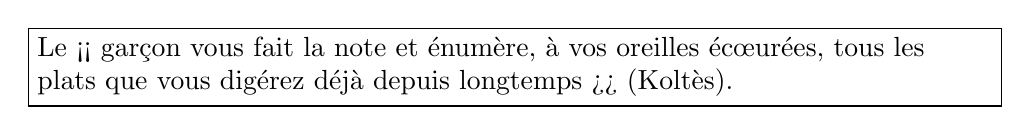
\begin{tikzpicture}
\node[draw, rectangle,text width=\textwidth] at (0,0) {Le << garçon vous fait la note et énumère, à vos oreilles écœurées, tous les plats que vous digérez déjà depuis longtemps >> (Koltès).};
\end{tikzpicture}
\end{frame}

%---------------------------------------------------------------------------------------------------------------------------------------- 
\begin{frame}[fragile]{\texttt{Packages} utiles}

\begin{itemize}
	\item \texttt{graphicx}
	\begin{itemize}
		\item Améliore la capacité d'inclusion d'images (pdf, png, jpg, \ldots)
	\end{itemize}
	\item \texttt{tabularx}
	\begin{itemize}
		\item Améliore la capacité de création de tableaux
	\end{itemize}
	\item \texttt{tikz}
	\begin{itemize}
		\item Permet la création de graphiques et animations vectoriels directement en code latex
	\end{itemize}
	\item \texttt{hyperref}
	\begin{itemize}
		\item Pour la gestion des hyper-liens externes et internes au document
	\end{itemize}
\end{itemize}
\end{frame}

%---------------------------------------------------------------------------------------------------------------------------------------- 
\begin{frame}[fragile]{Structure d'un document}

\begin{itemize}
	\item Tout document est composé de diverses sections hiérarchiques
	\item Commandes
	\begin{itemize}
		\item \verb+\part{titre}+
		\item \verb+\chapter{titre}+ (seulement \texttt{book} et \texttt{report})
		\item \verb+\section{titre}+
		\item \verb+\subsection{titre}+
		\item \verb+\subsubsection{titre}+
		\item \verb+\paragraph{titre}+
		\item \verb+\subparagraph{titre}+
	\end{itemize}
\end{itemize}
\end{frame}

%---------------------------------------------------------------------------------------------------------------------------------------- 
\begin{frame}[fragile]{Structure d'un document}

\begin{itemize}
	\item Chaque commande génère un numéro (\texttt{.aux}) et produit une entrée dans la table des matières (\texttt{.toc})
	\begin{itemize}
		\item Sauf les versions « * »
	\end{itemize}
		\item Commande
	\begin{itemize}
		\item \verb+\tableofcontents+
	\end{itemize}
\end{itemize}

\begin{center}
	\begin{tikzpicture}[overlay,node distance=1.5cm, every node/.style={fill=white, font=\sffamily},xshift=3cm,yshift=1cm,  align=center]
	% Specification of nodes (position, etc.)
	\node (tex)			[file] 							{source .tex};
	\node (compile)     [run, below of=tex, yshift=-1cm]          	{Compilateur \texttt{pdflatex}};
	\node (aux)     	[file, left of=compile, xshift=-2cm, text width=1cm]   		{.aux .toc};

	\draw[->] (tex.south) -- (compile.north);
	\draw[->] (compile.west) -- (aux.east);
	\draw[->] (aux) -- +(0,1) -- +(3.5,1) -- (compile.north);
	\end{tikzpicture}
\end{center}
\end{frame}

%---------------------------------------------------------------------------------------------------------------------------------------- 
\begin{frame}[fragile]{Références et renvois}

\begin{itemize}
	\item Une référence est définie par la commande \verb+\label{nom}+ qui associe l’étiquette nom au dernier numéro généré
	\item Le numéro associé à l’étiquette nom est généré par l’utilisation de la commande \verb+\ref{nom}+
	\item Le numéro de page associé à l’étiquette nom est généré par l’utilisation de la commande \verb+\pageref{nom}+
\end{itemize}
\end{frame}


%---------------------------------------------------------------------------------------------------------------------------------------- 
\begin{frame}[fragile]{Références}

\begin{verbatim}
\documentclass{report}
\usepackage[utf8]{inputenc}
\usepackage[T1]{fontenc}
\usepackage[french]{babel}
\begin{document}
\chapter{Gaston Miron} \label{s:miron}
\section{Notice biographique} \label{s:biogr}

Gaston Miron est né en 1928 à Sainte-Agathe-des-Monts: 
<< Je suis né ton fils en-haut là-bas dans les vieilles 
montagnes râpées du nord >> (L'Octobre).

Le chapitre~\ref{s:miron} inclut une brève 
notice biographique (\S\ref{s:biogr}) sur la vie 
de Gaston Miron.
\end{document}
\end{verbatim}
\end{frame}

%---------------------------------------------------------------------------------------------------------------------------------------- 
\begin{frame}[fragile]{Références}
\includegraphics[trim={4cm 5cm 4cm 6cm},clip,width=\textwidth]{ex_Ref}
\end{frame}

%---------------------------------------------------------------------------------------------------------------------------------------- 
\begin{frame}[fragile]{Notes de bas de page}

\begin{itemize}
	\item La commande \verb+\footnote{Texte de la note.}+ permet de placer une note en bas de page
\end{itemize}
\begin{verbatim}
Gaston Miron ... >> (L'Octobre\footnote{Ce poème est 
tiré du recueil \emph{L'Homme rapaillé} publié aux 
Presses de l'Université de Montréal en 1970.}).
\end{verbatim}
\vfill
\includegraphics[trim={4.5cm 14cm 4.5cm 12cm},clip,width=\textwidth]{ex_Ref}
\vfill
\includegraphics[trim={4.5cm 2cm 4.5cm 23cm},clip,width=\textwidth]{ex_Ref}
\end{frame}

%---------------------------------------------------------------------------------------------------------------------------------------- 
\begin{frame}[fragile]{Listes}

\begin{itemize}
	\item \begin{verbatim}
		\begin{liste}
		\item premier élément
		\item second élément
		...
		\item dernier élément
		\end{liste}
	\end{verbatim}
	\item Types de listes : 
	\begin{itemize}
		\item \texttt{itemize} : liste à items non numérotés
		\item \texttt{enumerate} : liste à items numérotés
		\item \texttt{description} : liste descriptive
	\end{itemize}
\end{itemize}
\end{frame}

%---------------------------------------------------------------------------------------------------------------------------------------- 
\begin{frame}[fragile]{Listes}

{\scriptsize
\begin{verbatim}
\begin{document}
	Voici trois exemples de listes. On y retrouve une 
	liste sans numérotation, une liste avec numérotation 
	et finalement une liste avec description.
	
	\begin{itemize}
		\item en français, les premiers éléments d'une 
		liste se terminent par un point virgule;
		\item chaque élément commence par une minuscule;
		\item le dernier élément a un point.
	\end{itemize}
	
	\begin{enumerate}
		\item L’hydrogène est le 1\ier{} élément.
		\item L’hélium est le 2\ieme{} élément.
		\item Le lithium est le 3\ieme{} élément.
	\end{enumerate}
	
	\begin{description}
		\item[Mercure] a un flux de rayonnement solaire de 9126.6~W/m$^2$.
		\item[Vénus] a un flux de rayonnement solaire de 2613.9~W/m$^2$.
		\item[Terre] a un flux de rayonnement solaire de 1367.6~W/m$^2$.
	\end{description}
\end{document}	
\end{verbatim}
}

\end{frame}

%---------------------------------------------------------------------------------------------------------------------------------------- 
\begin{frame}[fragile]{Listes}
\includegraphics[trim={4cm 12cm 4cm 3cm},clip,width=\textwidth]{ex_List}
\end{frame}

%---------------------------------------------------------------------------------------------------------------------------------------- 
\begin{frame}[fragile]{Tableaux}
\begin{itemize}
	\item Environnements : 
	\begin{itemize}
	\item \texttt{tabular} : mode texte 
	\item \texttt{array} : mode math
	\end{itemize}	
	\item \begin{verbatim}
	\begin{tabular}[position]{colonnes}
	... \\% rangée #1
	... \\% rangée #2
	\end{tabular}
	\end{verbatim}
	\item Positionnement vertical 
	\begin{itemize}
		\item centré par défaut
		\item \texttt{position} : \texttt{t} (<< top >>) | \texttt{b} (<< bottom >>) | \texttt{h} (<< here >>)
	\end{itemize}
\end{itemize}
\end{frame}

%---------------------------------------------------------------------------------------------------------------------------------------- 
\begin{frame}[fragile]{Tableaux}

Définition des colonnes :
\begin{itemize}
	\item \texttt{l} : left
	\item \texttt{r} : right
	\item \texttt{c} : center
	\item \texttt{|} : ligne verticale
	\item \texttt{p\{largeur\}} : paragraphe
	\begin{itemize}
		\item \texttt{largeur} : dimension de césure 
		\item e.g. : \texttt{0.5in | 1.27cm | 12.7mm | 36pt
}
	\end{itemize}	
\end{itemize}
\end{frame}

%---------------------------------------------------------------------------------------------------------------------------------------- 
\begin{frame}[fragile]{Tableaux}

\begin{itemize}
	\item \verb+&+ : séparateur de colonnes
	\item \verb+\\+ : indicateur de nouvelle rangée
	\item \verb+\hline+ : ligne horizontale
	\item \verb+\multicolumn{num}{col}{item}+ : permet de remplacer le format de \texttt{num} colonnes du tableau par une colonne de format \texttt{col} ayant le contenu \texttt{item}
\end{itemize}
\end{frame}


%---------------------------------------------------------------------------------------------------------------------------------------- 
\begin{frame}[fragile]{Tableaux}

{\scriptsize
	\begin{verbatim}
	\newcommand\centh[1]{\multicolumn{1}{c}{#1}}
	\begin{document}
	\begin{tabular}{p{5cm}lc}
	\hline
	\hline
	\centh{\emph{grandeur dérivée}} & \centh{\emph{nom}} & \emph{symbole} \\ 
	\hline
	différence de potentiel électrique, force électromotrice & volt  & V  \\
	puissance, flux énergétique                              & watt  & W  \\
	énergie, travail, quantité de chaleur                    & joule & J  \\ 
	\hline
	\hline
	\end{tabular}
	\end{document}
	\end{verbatim}
}

\end{frame}

%---------------------------------------------------------------------------------------------------------------------------------------- 
\begin{frame}[fragile]{Tableaux}
\begin{center}
	\includegraphics[trim={4cm 12cm 6cm 3cm},clip,width=\textwidth]{ex_Tab}	
\end{center}
\end{frame}

%---------------------------------------------------------------------------------------------------------------------------------------- 
\begin{frame}[fragile]{Tableaux ++}

\begin{itemize}
	\item Package \texttt{array} : \url{https://ctan.org/pkg/array}
	\begin{itemize}
		\item  Définitions de colonnes supplémentaires
	\end{itemize}
	\item Package \texttt{longtable} : \url{https://ctan.org/pkg/longtable}
	\begin{itemize}
		\item  Tableau sur plusieurs pages
	\end{itemize}
	\item Package \texttt{multirow} : \url{https://ctan.org/pkg/multirow}
	\begin{itemize}
		\item  Version horizontale de \verb+\multicolumn+
	\end{itemize}
	\item Package \texttt{tabularx} : \url{https://ctan.org/pkg/tabularx}
	\begin{itemize}
		\item  Colonne X pour une colonne p qui complète à \verb+\textwidth+
	\end{itemize}
	\item Package \texttt{dcolumn} : \url{https://ctan.org/pkg/dcolumn}
	\begin{itemize}
		\item  pour aligner les valeurs numériques sur le "."
	\end{itemize}
	\item \href{https://texblog.org/2017/02/06/proper-tables-with-latex/}{... and other fancy tables}\footnote{it's a link !}
\end{itemize}

\end{frame}

%---------------------------------------------------------------------------------------------------------------------------------------- 

\begin{frame}[fragile]{Objets graphiques}

\begin{itemize}
	\item Package \texttt{graphicx}
	\item \verb+\includegraphics[cle=val,...,cle=val]{fichier}+
	\begin{itemize}
		\item Insère un fichier graphique
		\item Formats supportés par le compilateur latex : eps | tiff
		\item Formats supportés par le compilateur pdflatex : pdf | jpg | png
		\item Toujours utiliser des chemins relatifs
	\end{itemize}	
\end{itemize}
\end{frame}

%---------------------------------------------------------------------------------------------------------------------------------------- 
\begin{frame}[fragile]{Objets graphiques}

{\LARGE \texttt{cle=valeur}}
\begin{itemize}
	\item Paramètres optionnels
	\item Liste de paires
	\item Séparés par des virgules
	\begin{itemize}
		\item \texttt{width} : largeur de la figure
		\item \texttt{height} : hauteur de la figure
		\item \texttt{scale} : facteur d’échelle
		\item \texttt{angle} : angle de rotation (sens horaire)
		\item \texttt{origin} : origine pour la rotation
		\item \texttt{viewport} : 4 paramètres de la « bounding box »
		\item \texttt{trim} : 4 paramètres pour déplacer les marges
		\item etc.
	\end{itemize}	
\end{itemize}
\centering\footnotesize \verb+\includegraphics[trim={4cm 12cm 6cm 3cm},clip,width=\textwidth]{ex_Tab}+
\end{frame}

%---------------------------------------------------------------------------------------------------------------------------------------- 
\begin{frame}[fragile]{Objets flottants}
\begin{itemize}
	\item Objets dont la localisation est déterminée par le compilateur
	\item Permettent l'ajout d'une légende et d'une référence
	\begin{itemize}
	\item \verb+\caption{legende}+
	\item \verb+\label{nom}+
	\end{itemize}
	\item Environnement de tableau
: \texttt{table}
	\begin{verbatim}
	\begin{table}[localisation] \end{table}
	\end{verbatim}
	\item Environnement d'image
: \texttt{figure}
	\begin{verbatim}
	\begin{figure}[localisation] \end{figure}
	\end{verbatim}
	\item Localisation :
	\begin{itemize}
		\item \texttt{h} : ici (« here »)
		\item \texttt{t} : haut de page (« top »)
		\item \texttt{b} : bas de page (« bottom »)
		\item \texttt{p} : page dédiée aux objets flottants (« page of floats »)
		\item \texttt{tbp} : défaut
		\item \texttt{!htb} : recommandé
	\end{itemize}

\end{itemize}
\end{frame}

%---------------------------------------------------------------------------------------------------------------------------------------- 
\begin{frame}[fragile]{Objets flottants}
\begin{itemize}
	\item Chaque commande \verb+\caption+ génère un numéro (\texttt{.aux}) et produit une entrée dans la liste des tableaux (\texttt{.lot}) / la liste des figures (\texttt{.lof})
	\item Commande \verb+\listoffigures+
	\item Commande \verb+\listoftables+
\end{itemize}
\begin{center}
	\begin{tikzpicture}[overlay,node distance=1.5cm, every node/.style={fill=white, font=\sffamily},xshift=3cm,yshift=1cm,  align=center]
	% Specification of nodes (position, etc.)
	\node (tex)			[file] 							{source .tex};
	\node (compile)     [run, below of=tex, yshift=-1cm]          	{Compilateur \texttt{pdflatex}};
	\node (aux)     	[file, left of=compile, xshift=-2cm, text width=1cm]   		{.aux .toc .lof .lot};
	
	\draw[->] (tex.south) -- (compile.north);
	\draw[->] (compile.west) -- (aux.east);
	\draw[->] (aux) -- +(0,1) -- +(3.5,1) -- (compile.north);
	\end{tikzpicture}
\end{center}

\end{frame}

\begin{frame}[fragile]{Objets flottants}

\tiny
\begin{Verbatim}
\documentclass[french]{article}
\usepackage[utf8]{inputenc}
\usepackage{babel}
\usepackage{graphicx}
\usepackage{caption}
\DeclareCaptionLabelSeparator{as-Babel-french}{\space\textendash\space}
\captionsetup{labelsep=as-Babel-french}
\captionsetup[table]{position=top}
\newcommand\multi[2]{\multicolumn{1}{#1}{#1}}
\begin{document}
Le tableau~\ref{t:prix_materiaux} et la figure~\ref{f:echantillons} illustrent l'utilisation 
d'objets flottants qui sont positionnés immédiatement après le texte. Comme il se doit dans 
un texte en français, la légende du tableau le précède, alors que celle de la figure la suit.
	\begin{table}[htp] \caption{Liste de prix des matériaux de référence au 1 février 2006, minérales (LMSM).}
	\centering
	\label{t:prix_materiaux}
		\begin{tabular}{|l|c|r|} \hline\hline
			\multi{|c|}{\emph{description}} & \emph{unité} & \multi{c|}{\emph{prix}}
			\\ \hline
			Minerai d'uranium          & 100 g     &   95,00  \$ \\
			Minerai d'or               & 200 g     &  180,00  \$ \\
			Alliages de zinc-aluminium & 7 disques & 1500,00 \$ \\
			\hline\hline
		\end{tabular}
	\end{table}
	\begin{figure} % top par défaut
	\centering
		\includegraphics[width=0.5\textwidth]{mat}
		\caption{Les matériaux de référence se présentent sous forme d'échantillons en
		poudre de minerais, de roches, de sédiments, de sols, de concentrés et de
		produits de traitement, dont la composition chimique a été établie avec
		précision.} 		\label{f:echantillons}
	\end{figure}
\end{document}
\end{Verbatim}
\end{frame}

%---------------------------------------------------------------------------------------------------------------------------------------- 
\begin{frame}[fragile]{Objets flottants}
\begin{center}
	\includegraphics[trim={3cm 5cm 3cm 5cm},clip,width=\textwidth, scale=0.5]{ex_Float}	
\end{center}
\end{frame}

%---------------------------------------------------------------------------------------------------------------------------------------- 
\begin{frame}[fragile]{Objets flottants ++}
\begin{itemize}
	\item Package \texttt{rotating} : \url{https://ctan.org/pkg/rotating}
	\begin{itemize}
		\item  Format paysage
		\item  Environnement sidewaystable 
		\item  Environnement sidewaysfigure
	\end{itemize}
	\item Package \texttt{caption} : \url{https://ctan.org/pkg/caption}
	\begin{itemize}
		\item Redéfinition aisée des paramètres
		\item Relocalisation (haut vs bas)	
	\end{itemize}
	\item Package \texttt{subfig} : \url{https://ctan.org/pkg/subfig}
	\begin{itemize}
		\item  Usage de sous-figures / sous-tableaux
	\end{itemize}
\end{itemize}

\end{frame}

%---------------------------------------------------------------------------------------------------------------------------------------- 
\begin{frame}[fragile]{Mode Mathématique}

\begin{itemize}
\item  Style « texte » : formules intégrées au texte
\begin{itemize}
\item \verb+$...$+
\end{itemize}
\item  Style « affichage » : formules centrées et intercalées entre paragraphes (displaystyle)
\begin{itemize}
\item \verb+$$ ... $$+
\end{itemize}
\item  Style « affichage » : formules centrées et intercalées entre paragraphes, numérotées (avec ref possible)
\begin{itemize}
\item \verb+\begin{equation} ... \end{equation}+
\end{itemize}
\end{itemize}
\end{frame}

%---------------------------------------------------------------------------------------------------------------------------------------- 
\begin{frame}[fragile]{Mode Mathématique}
\tiny
\begin{Verbatim}
Le déploiement simple d'expressions mathématiques complexes est une des grandes forces de \LaTeX. 
Il est tout aussi aisé d'insérer une équation en mode texte (<< text style >>), donc qui s'intègre dans 
un paragraphe, telles que $V=RI$ ou $\mathbf{b} = \mathbf{A} \mathbf{x}$, que des équations en 
mode d'affichage hors texte (<< display style >>) sans numérotation,
$$ b_i = \sum_{j=1}^{2} a_{ij} x_{j}, $$

ou encore avec numérotation, telle que l'éq.~(\ref{eq:matrice}):
\begin{equation}
	\left[ \begin{array}{c} b_{1} \\ b_{2} \end{array} \right]
		= \left[ \begin{array}{cc} a_{11} & a_{12} \\ a_{21} & a_{22} \end{array} \right]
		\times
		\left[ \begin{array}{c} x_{1} \\ x_{2} \end{array} \right].
	\label{eq:matrice}
\end{equation}

L'équation affichée sans numérotation ne possède évidemment pas de numéro, on ne peut donc ni 
y définir une référence dynamique, ni y référer.

\end{Verbatim}
\end{frame}

%---------------------------------------------------------------------------------------------------------------------------------------- 
\begin{frame}[fragile]{Mode Mathématique}
\small

Le déploiement simple d'expressions mathématiques complexes est une des grandes forces de \LaTeX. 
Il est tout aussi aisé d'insérer une équation en mode texte (<<~text style~>>), donc qui s'intègre dans 
un paragraphe, telles que $V=RI$ ou $\mathbf{b} = \mathbf{A} \mathbf{x}$, que des équations en 
mode d'affichage hors texte (<<~display style~>>) sans numérotation,
$$ b_i = \sum_{j=1}^{2} a_{ij} x_{j},$$


ou encore avec numérotation, telle que l'éq.~(\ref{eq:matrice}):
\begin{equation}
\left[ \begin{array}{c} b_{1} \\ b_{2} \end{array} \right]
= \left[ \begin{array}{cc} a_{11} & a_{12} \\ a_{21} & a_{22} \end{array} \right]
\times
\left[ \begin{array}{c} x_{1} \\ x_{2} \end{array} \right].
\label{eq:matrice}
\end{equation}

L'équation affichée sans numérotation ne possède évidemment pas de numéro, on ne peut donc ni 
y définir une référence dynamique, ni y référer.

\end{frame}

%---------------------------------------------------------------------------------------------------------------------------------------- 
\begin{frame}[fragile]{Citations et Bibliographie}

L'énorme avantage de \LaTeX sur les WYSIWYG:
\begin{itemize}
	\item  Un fichier qui regroupe de manière structurée les ouvrages à citer (articles de journaux et conférences, livres, thèses, etc.)
	\begin{itemize}
		\item \verb+@type{clé, champ1={val1},champ2={val2},...}+
		\item Au format directement téléchargeable sur Google Scholar, Arxiv, ou autre.
		\item La gestion de ces références peut-être par des logiciels de type \href{http://www.jabref.org/}{JabRef}.
	\end{itemize}
	\item Une inclusion du fichier bibliography à la fin du document pour déclarer les références
	\begin{itemize}
		\item \verb+\bibliography{file}+ : Pour le fichier \texttt{file.bib}
	\end{itemize}
	\item  Citation dans le texte en utilisant la clé
	\begin{itemize}
		\item \verb+\cite[texte]{cle}+ : texte optionnel pour le numéro de chapitre, ou de paragraphe.
	\end{itemize}
	\item  Changement du style de citation en une seule ligne : 
	\begin{itemize}
	\item \verb+\bibliographystyle{type}+ : type : \texttt{alpha | apalike | ieeetr | plain | ...}
\end{itemize}
\end{itemize}
\end{frame}

%---------------------------------------------------------------------------------------------------------------------------------------- 
\begin{frame}[fragile]{Citations et Bibliographie}
\tiny
\begin{Verbatim}
%%%%%%%%%%%%
% File ex_Bib.bib

@book{BOOK:1,
AUTHOR={John Doe},
TITLE={The Book without Title},
PUBLISHER={Dummy Publisher},
YEAR={2100},
}
@article{ARTICLE:1,
AUTHOR={John Doe and Wallace Gromit},
TITLE={Title},
JOURNAL={Journal},
YEAR={2019},
}
@inproceedings{CONF:1,
author = {John Doe, Arthur Smith and Wallace Gromit},
title = {Title},
booktitle = {Proc~.of the XXth Inter. Conf. on Machine learning (ICML)},
year = {2019},
pages = {AAA--BBB}
}

%%%%%%%%%%%%
% File ex_Bib.tex

\documentclass{article}
\begin{document}
Citation random~\cite{BOOK:1} dans~\cite{ARTICLE:1} le texte~\cite{CONF:1}.
\bibliography{ex_Bib} 
\bibliographystyle{ieeetr}
\end{document}
\end{Verbatim}
\end{frame}

%---------------------------------------------------------------------------------------------------------------------------------------- 
\begin{frame}[fragile]{Citations et Bibliographie}
\begin{center}
	\includegraphics[trim={3cm 3cm 3cm 3cm},clip,width=\textwidth]{ex_Bib}	
\end{center}
\end{frame}

%---------------------------------------------------------------------------------------------------------------------------------------- 
\begin{frame}[fragile]{Citations et Bibliographie ++}

\begin{itemize}
	\item Package \texttt{rotating} : \url{https://ctan.org/pkg/rotating}
	\begin{itemize}
		\item  Format paysage
		\item  Environnement sidewaystable 
		\item  Environnement sidewaysfigure
	\end{itemize}
	\item Package \texttt{caption} : \url{https://ctan.org/pkg/caption}
	\begin{itemize}
		\item Redéfinition aisée des paramètres
		\item Relocalisation (haut vs bas)	
	\end{itemize}
	\item Package \texttt{subfig} : \url{https://ctan.org/pkg/subfig}
	\begin{itemize}
		\item  Usage de sous-figures / sous-tableaux
	\end{itemize}
\end{itemize}

\end{frame}

%---------------------------------------------------------------------------------------------------------------------------------------- 
\begin{frame}[fragile]{Inclusions de fichiers}

Pour une meilleure gestion des versions, lisibilité du code, réutilisation, vitesse de compilation : 
\begin{itemize}
	\item Inclusion d’un fichier comme s’il était dans le texte
	\begin{itemize}
		\item \verb+\input{fichier}+
		\item Utile pour les figures Tikz, les macros réutilisables 
		\item Peut lui même contenir des \verb+\input{}+
	\end{itemize}
	
	\item Inclusion de chapitres complets
	\begin{itemize}	
		\item \verb+\include{chapitre}+
		\item Création d’un fichier chapitre.aux supplémentaire : recompilation accélérée
		\item \verb+\includeonly{...}+ : pour valider si le ficher existe
		\item Utile pour les gros travaux découpés ou collaboratifs
		\item Mais force le changement de page avant et après, et ne peut contenir d'autre \verb+\include{}+
	\end{itemize}
\end{itemize}
\end{frame}

%---------------------------------------------------------------------------------------------------------------------------------------- 
\begin{frame}[fragile]{Hyperliens et URLs}

Package \texttt{hyperref}
\begin{itemize}
	\item Conversion automatique de toutes les références en hyperliens internes au document
	\item Commande \verb+\url{lien}+
	\item Commande \verb+\href{url}{text}+
	\begin{itemize}
		\item URL : « Uniform Resource Locator »
	\end{itemize}
\end{itemize}
\end{frame}

%---------------------------------------------------------------------------------------------------------------------------------------- 


\section{Beamer}
% Nécessaire pour afficher du code beamer dans beamer
\newenvironment{fragileframe}{\begin{frame}[fragile,environment=fragileframe]}{\end{frame}}

%---------------------------------------------------------------------------------------------------------------------------------------- 

\begin{frame}[fragile]{Beamer : Présentations}
\begin{itemize}
	\item \texttt{Beamer} est une classe de \LaTeX permettant de réaliser des présentations ou diaporamas au format pdf.
	\item Il propose de nombreux thèmes de présentations donnant une apparence soignée et agréable.
	\item Beamer est basé sur un environnement de page (\texttt{frame}) qui représente une "acétate", laquelle peut être affichée en plusieurs étapes par une succession de couches (\texttt{slides}).
\end{itemize}
La compilation s’effectue comme pour un document \LaTeX standard. Toutes les commandes \LaTeX, ou presque, sont acceptées parBeamer.
\end{frame}

%---------------------------------------------------------------------------------------------------------------------------------------- 

\begin{frame}[fragile]{Préambule}
Il est possible de personnaliser complètement l’apparence de son diaporama mais recommandé pour débuter d’utiliser les thèmes fournis avec Beamer. Ceux-ci se divisent en cinq grandes catégories :
\begin{description}
	\item[Thème de présentation globale] qui gère la totalité du diaporama
	\item[Thème de couleur] permettant de modifier les couleurs de base d’un thème global ou une partie seulement des couleurs selon les thèmes.
	\item[Thème de police] gère tout ce qui est relatif aux polices : gras, italique,...
	\item[Thème interne] gère l’apparence des éléments tels que les listes, la tabledes matières, les notes, la bibliographie,...
	\item[Thème externe] gère les en-têtes et pieds-de-page, le titre de la page, lelogo, la barre de navigation,...
\end{description}
\end{frame}


%---------------------------------------------------------------------------------------------------------------------------------------- 
\begin{frame}[fragile]{Préambule}
Le choix des thèmes précédents se fait dans le préambule par :
{\footnotesize
\begin{Verbatim}
\usetheme{nom du theme global}
\usecolortheme{nom du theme de couleur}
\usefonttheme{nom du theme de police}
\useinnertheme{nom du theme interne}
\useoutertheme{nom du theme externe}
\end{Verbatim}
}
On a utilisé ici : 
{\footnotesize
	\begin{Verbatim}
\usepackage{../beamerthemeulaval}
\usepackage{../beamercolorthemeulaval}
\end{Verbatim}
}
\end{frame}

%---------------------------------------------------------------------------------------------------------------------------------------- 

\begin{fragileframe}{Page : \texttt{frame}}
	Le titre d'une page est affiché en haut de la page dans une taille plus importante. Sa couleur et son fond dépendent du thème choisi.
	Le sous-titre éventuel d'une page est plus petit que le titre et apparaît juste en-dessous.
	\footnotesize
	\begin{Verbatim}
	\begin{frame}[options]
		\frametitle{Ceci est le titre}
		\framesubtitle{Ceci est le sous-titre}
		Contenu de la page
	\end{frame}
	\end{Verbatim}
\end{fragileframe}

%---------------------------------------------------------------------------------------------------------------------------------------- 


\begin{fragileframe}{Page : \texttt{frame}}
	
	Options possibles
	\begin{description}
		\item[plain] les entêtes, pieds de pages et panneaux latéraux sont supprimés de la diapo. On peut donc localement en ajouter de nouveaux ou bien mettre une figure qui tient sur la diapo complète.
		\item[fragile] utilisée lorsque du code qui ne doit pas être compilé comme tel est inséré (exemple : environnement \texttt{verbatim})
		\item[label=nom] le contenu de la diapo est enregistrée sous ce label etpeut donc être rappélée avec la commande \verb+\againframe+.
		\item[...]
	\end{description}
\end{fragileframe}


%---------------------------------------------------------------------------------------------------------------------------------------- 
\begin{fragileframe}{Page de titre}
\footnotesize
	\begin{Verbatim}
\begin{frame}[label=titre, plain]
\titlepage
\begin{center}
	\includegraphics[height=1cm]{UL_P}
\end{center}
\end{frame}
	\end{Verbatim}
\end{fragileframe}

%---------------------------------------------------------------------------------------------------------------------------------------- 

\begin{fragileframe}{Sections}
Il est possible de faire apparaître le sommaire à différents endroits et de manière automatique :
{\footnotesize
\begin{Verbatim}
\AtBeginSection[]{
\begin{frame}
	\Huge \centerline{\insertsection}
	%  \small \tableofcontents[currentsection, hideothersubsections]
\end{frame} 
}
\end{Verbatim}
}
\begin{itemize}
	\item \texttt{section} crée une page de transition avec le titre (et les sous-sections)
	\item \texttt{subsection} et \texttt{subsubsection} sont utiles pour le sommaire seulement
\end{itemize}
{\footnotesize
	\begin{Verbatim}
\section{Main Section}

\subsection{List styles}

\subsubsection{Itemize}
	\end{Verbatim}
}
\end{fragileframe}

%---------------------------------------------------------------------------------------------------------------------------------------- 

\begin{fragileframe}{Page d'outline}
	\footnotesize
	\begin{Verbatim}
	\begin{frame}[label=toc]{Outline}
	\setlength{\leftskip}{5cm}%
	\tableofcontents[subsectionstyle=show]
	\end{frame}
	\end{Verbatim}
\end{fragileframe}


%---------------------------------------------------------------------------------------------------------------------------------------- 

\begin{fragileframe}{Listes : \texttt{itemize}}
	\footnotesize
	\begin{Verbatim}
\begin{frame}[label=itemize]\frametitle{Itemize sample} 
\begin{itemize}
	\item Item 1
	\item Item 2
	\begin{itemize}
		\item Sub item 1
		\item Sub item 2
		\begin{itemize}
			\item Sub sub sub item 1
			\item Sub sub sub item 2
		\end{itemize}
		\item Sub item 3
	\end{itemize}
	\item Item 3
\end{itemize}
\end{frame}
	\end{Verbatim}
\end{fragileframe}

%---------------------------------------------------------------------------------------------------------------------------------------- 
\begin{frame}[label=itemize]\frametitle{Itemize sample} 
\begin{itemize}
	\item Item 1
	\item Item 2
	\begin{itemize}
		\item Sub item 1
		\item Sub item 2
		\begin{itemize}
			\item Sub sub sub item 1
			\item Sub sub sub item 2
		\end{itemize}
		\item Sub item 3
	\end{itemize}
	\item Item 3
\end{itemize}
\end{frame}

%---------------------------------------------------------------------------------------------------------------------------------------- 
\begin{fragileframe}{Listes : \texttt{enumerate}}
	\footnotesize
	\begin{Verbatim}
\begin{frame}[label=enumerate]\frametitle{Enumerate sample} 
\begin{enumerate}
	\item Item 1
	\item Item 2
	\begin{enumerate}
		\item Sub item 1
		\item Sub item 2
		\begin{enumerate}
			\item Sub sub sub item 1
			\item Sub sub sub item 2
		\end{enumerate}
		\item Sub item 3
	\end{enumerate}
	\item Item 3
\end{enumerate}
\end{frame}
	\end{Verbatim}
\end{fragileframe}

%---------------------------------------------------------------------------------------------------------------------------------------- 

\begin{frame}[label=enumerate]\frametitle{Enumerate sample} 
	\begin{enumerate}
	\item Item 1
	\item Item 2
	\begin{enumerate}
	\item Sub item 1
	\item Sub item 2
	\begin{enumerate}
	\item Sub sub sub item 1
	\item Sub sub sub item 2
	\end{enumerate}
	\item Sub item 3
	\end{enumerate}
	\item Item 3
	\end{enumerate}
\end{frame}


%---------------------------------------------------------------------------------------------------------------------------------------- 
\begin{fragileframe}{Listes : \texttt{description}}
	\footnotesize
	\begin{Verbatim}

\begin{frame}[label=description]\frametitle{Description sample}

\begin{description}
	\item[Term 1:] Definition 1
	\item[Term 2:] Definition 2
	\item[Term 3:] Definition 3
\end{description}
\end{frame}

	\end{Verbatim}
\end{fragileframe}

%---------------------------------------------------------------------------------------------------------------------------------------- 
\begin{frame}[label=description]\frametitle{Description sample}
	
	\begin{description}
	\item[Term 1:] Definition 1
	\item[Term 2:] Definition 2
	\item[Term 3:] Definition 3
	\end{description}
\end{frame}
	

%---------------------------------------------------------------------------------------------------------------------------------------- 
\begin{fragileframe}{Boites}
	\footnotesize
	\begin{Verbatim}
	
\begin{frame}[label=boxes]\frametitle{Boxes Styles}

	\begin{block}{Block Title}
	Block content
	\end{block}
	
	\begin{alertblock}{Alert Block Title}
	Alert block content
	\end{alertblock}
	
	\begin{exampleblock}{Example Block Title}
	Example block content
	\end{exampleblock}

\end{frame}

\end{Verbatim}
\end{fragileframe}

%---------------------------------------------------------------------------------------------------------------------------------------- 
\begin{frame}[label=boxes]\frametitle{Boxes Styles}

\begin{block}{Block Title}
	Block content
\end{block}

\begin{alertblock}{Alert Block Title}
	Alert block content
\end{alertblock}

\begin{exampleblock}{Example Block Title}
	Example block content
\end{exampleblock}

\end{frame}


%---------------------------------------------------------------------------------------------------------------------------------------- 
\begin{fragileframe}{Environnements spéciaux}
	\footnotesize
	\begin{Verbatim}
	
\begin{frame}[label=environments]\frametitle{Environments Samples}

	\begin{definition}
	Definition content
	\end{definition}
	
	\begin{example}
	Example content
	\end{example}
	
	\begin{proof}
	Proof content
	\end{proof}  
	
	\begin{theorem}
	Theorem content
	\end{theorem}

\end{frame}
	\end{Verbatim}
\end{fragileframe}


%---------------------------------------------------------------------------------------------------------------------------------------- 
\begin{frame}[label=environments]\frametitle{Environments Samples}

\begin{definition}
	Definition content
\end{definition}

\begin{example}
	Example content
\end{example}

\begin{proof}
	Proof content
\end{proof}  

\begin{theorem}
	Theorem content
\end{theorem}

\end{frame}

%---------------------------------------------------------------------------------------------------------------------------------------- 
\begin{fragileframe}{Deux colonnes}
	
	L’environnement \texttt{minipage} est pour cela très pratique. Par exemple pour mettre deux figures côté à côte, ou bien une légende à côté d’une figure :
	\footnotesize
	\begin{Verbatim}
\begin{minipage}[c]{0.45\textwidth}
	\fbox{\includegraphics[width=\textwidth]{exemple}}
\end{minipage}
\hfill
\begin{minipage}[c]{0.45\textwidth}
	Ici la légende de la figure
\end{minipage}
	\end{Verbatim}
\end{fragileframe}

%---------------------------------------------------------------------------------------------------------------------------------------- 
\begin{fragileframe}{Deux colonnes}
	
	\begin{minipage}{0.55\textwidth}
%		\fbox{\includegraphics[width=\textwidth]{exemple}}
		\input{exemple.tikz}
	\end{minipage}
	\hfill
	\begin{minipage}{0.35\textwidth}
		Ici la légende de la figure
	\end{minipage}
\end{fragileframe}

%---------------------------------------------------------------------------------------------------------------------------------------- 

\begin{fragileframe}{Affichage séquentiel}
	
	Beamer permet de superposer différentes couches d’affichage. Voici un exemple :

	\begin{itemize}
	\item<1> Un premier élément
	\item<2-> Un deuxième éléement qui reste
	\item<3-> \textbf<4>{Un troisième élément qui 
	sera bientôt gras}
	\item<4> La fin.
	\end{itemize}

\end{fragileframe}

%---------------------------------------------------------------------------------------------------------------------------------------- 

\begin{fragileframe}{Affichage séquentiel}
	
	Beamer permet de superposer différentes couches d’affichage. Voici un exemple :
	\footnotesize
	\begin{Verbatim}
	\begin{itemize}
	\item<1> Un premier élément
	\item<2-> Un deuxième éléement qui reste
	\item<3-> \textbf<4>{Un troisième élément qui 
	sera bientôt gras}
	\item<4> La fin.
	\end{itemize}
	\end{Verbatim}
	
	Il est aussi possible de faire des overlay et des transitions ... mais je vous laisse chercher, parce que faire des animations, c'est long et souvent inutile.
\end{fragileframe}

%---------------------------------------------------------------------------------------------------------------------------------------- 
\section{PGF/TikZ}
%---------------------------------------------------------------------------------------------------------------------------------------- 
\renewcommand\arraystretch{1.5}

%---------------------------------------------------------------------------------------------------------------------------------------- 

\begin{fragileframe}{PGF and TikZ}
	\begin{itemize}
		\item Selon son auteur, Till Tantau (Lübeck), PGF / TikZ signifie «Portable Graphics Format» et «\emph{TikZ ist kein Zeichenprogramm}».
		\item PGF: moteur interne;
		\item TikZ: interface parfaitement intégrée dans \LaTeX et Beamer
		\item fonctionne pour la sortie PostScript (\texttt{dvips}) ainsi que pour la génération de PDF (\texttt{pdflatex}, \texttt{dvipdfmx})
		\item Les prévisualiseurs DVI ne sont pas toujours en mesure d’afficher correctement les graphiques. Vérifiez la sortie PS ou PDF.
	\end{itemize}
\end{fragileframe}

%---------------------------------------------------------------------------------------------------------------------------------------- 

\begin{fragileframe}{}
	\begin{itemize}
		\item \verb+\tikz+ peut être utilisé \emph{inline} :\\
		i.e. Le code \verb+\tikz{\draw (0pt,0pt) -- (20pt,6pt);}+ donne \tikz{\draw (0pt,0pt) -- (20pt,6pt);} et \verb+\tikz{\fill[orange] (0,0) circle (1ex);}+ donne \tikz{\fill[orange] (0,0) circle (1ex);}.
		\item L'environnement \verb+\begin{tikzpicture}...\end{tikzpicture}+ est utilisé pour des images plus grandes
	\end{itemize}
\vfill
	\begin{minipage}{0.19\textwidth}
	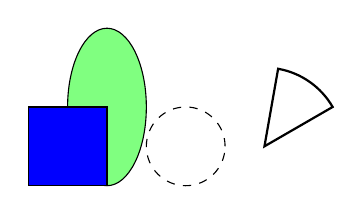
\begin{tikzpicture}
		\draw[style=dashed] (2,.5) circle (0.5);
		\draw[fill=green!50] (1,1)ellipse (.5 and 1);
		\draw[fill=blue] (0,0) rectangle (1,1);
		\draw[style=thick](3,.5) -- +(30:1) arc(30:80:1) -- cycle;
	\end{tikzpicture}
	\end{minipage}
	\hfill
	\begin{minipage}{0.79\textwidth}
	\scriptsize
	\begin{Verbatim}
		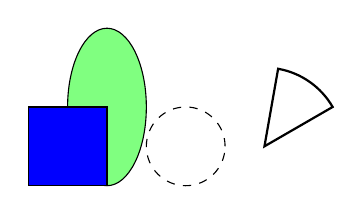
\begin{tikzpicture}
		\draw[style=dashed] (2,.5) circle (0.5);
		\draw[fill=green!50] (1,1)ellipse (.5 and 1);
		\draw[fill=blue] (0,0) rectangle (1,1);
		\draw[style=thick](3,.5) 
			-- +(30:1) arc(30:80:1) 
			-- cycle;
		\end{tikzpicture}
		\end{Verbatim}
	\end{minipage}

\end{fragileframe}

%---------------------------------------------------------------------------------------------------------------------------------------- 

\usetikzlibrary{backgrounds}
\begin{fragileframe}{}
	\begin{itemize}
		\item Les coordonées commencent dans le coin inférieur gauche du \texttt{canvas}
		\item Le \texttt{canvas} est construit de manière à contenir l'image
		\item Tip: affichez les limites du canvas, \\
		si nécessaire, déplacez l'image en \\
		utilisant \verb+\hspace*{..}, \vspace*{..}+
		\item Unité de longueur: \texttt{1cm}, d'autres unités \\
		possible (\texttt{pt}, \texttt{in}, ...)
		\item Tip: n'utilisez pas d'unités, utilisez l'option \\
		\texttt{scale} de la \texttt{tikzpicture}
	\end{itemize}

\vspace*{-2.3cm}\hspace{8cm}%
\begin{tikzpicture}[ scale=.8, show background rectangle]
\draw (2,2) circle (1);
\draw (1 mm, 10 pt) -- (4 em, 1);
\end{tikzpicture}

\scriptsize
	\begin{Verbatim}
\usetikzlibrary{backgrounds}
...
\vspace*{-2.3cm}\hspace{8cm}%
\begin{tikzpicture}[ scale=.8, show background rectangle]
\draw (2,2) circle (1);
\draw (1 mm, 10 pt) -- (4 em, 1);
\end{tikzpicture}
		\end{Verbatim}
\hrulefill

(Une solution dans l’esprit de \LaTeX serait l’utilisation d’un environnement \texttt{multicolumn} ou de \texttt{minipage}. Mais parfois, le hack \texttt{hspace} / \texttt{vspace} est plus rapide et plus flexible.)
\end{fragileframe}

%---------------------------------------------------------------------------------------------------------------------------------------- 


\begin{fragileframe}{Paths}
	\begin{itemize}
		\item Les éléments de base sont \texttt{paths} et \texttt{nodes}.
		\item Un \texttt{path} est une série de ligne droites et courbes.
		\item Les \texttt{paths} peuvent être \texttt{drawn}, \texttt{filled} ou utilisés comme \texttt{clipping} de dessins postérieurs:
	\end{itemize}

\begin{center}
		\begin{adjustbox}{max width=.7\textwidth}
	\begin{tabular}{cl}
		\tikz{\path[draw] (1,1) -- (2,2) -- (3,1);} & \verb+\path[draw] (1,1) -- (2,2) -- (3,1);+ \\
		\tikz{\path[draw,line width=4pt] (1,1) -- (2,2)--(3,1)--cycle;} & \verb+\path[draw,line width=4pt] (1,1) -- (2,2)--(3,1)--cycle;+\\
		\tikz{\path[draw, fill=green!20] (1,1)--(2,2)--(3,1)--cycle;} & \verb+\path[draw, fill=green!20] (1,1)--(2,2)--(3,1)--cycle;+\\
		\tikz{\path[fill=green] (1,1) -- (2,2) -- (3,1) -- cycle;} & \verb+\path[fill=green] (1,1) -- (2,2) -- (3,1) -- cycle;+\\
		\tikz{\path[clip, draw] (1,1)--(2,2)--(3,1)--cycle;} & \verb+\path[clip, draw] (1,1)--(2,2)--(3,1)--cycle;+\\
		\tikz{\path[fill=blue!50] (2, 1.7) circle (.8);} & \verb+\path[fill=blue!50] (2, 1.7) circle (.8);+\\
	\end{tabular}
	\end{adjustbox}
\end{center}	

	\begin{itemize}
		\item Abbreviations : \scriptsize
		\begin{Verbatim}
		\draw = \path[draw], \fill = \path[fill], 
		\clip = \path[clip], \filldraw = \path[fill,draw], 
		\shade = \path[shade], ...
		\end{Verbatim}
	\end{itemize}
	
\end{fragileframe}

%---------------------------------------------------------------------------------------------------------------------------------------- 
\newsavebox\myboxa
\begin{lrbox}{\myboxa}\begin{minipage}[t]{3in}
		\begin{verbatim}
\shade[shading=ball, ball color=blue]  (0,0) circle (.3);
\shade[shading=ball, ball color=white] (1,0) circle (.3);
\shade[shading=ball, ball color=black] (2,0) circle (.3);
		\end{verbatim}
\end{minipage}\end{lrbox}



\begin{fragileframe}{Shading}	
	\begin{center}
		\begin{adjustbox}{max width=\textwidth}
			\begin{tabular}{cl}
				\tikz{\path[shade,draw] (1,1) -- (2,2)--(3,1)--cycle;} & \verb+\path[shade,draw] (1,1) -- (2,2)--(3,1)--cycle;+ \\
				\tikz{\shade[left color=red] (1,1)--(2,2)--(3,1)--cycle;} & \verb+\shade[left color=red] (1,1)--(2,2)--(3,1)--cycle;+ \\
				\tikz{\shade[top color=red, bottom color=green](0,0) rectangle (2,1);} & \verb+\shade[top color=red, bottom color=green](0,0) rectangle (2,1);+ \\
				\tikz{\shade[draw,shading=radial, inner color=blue](0,0) rectangle (2,1);} & \verb+\shade[draw,shading=radial, inner color=blue](0,0) rectangle (2,1);+ \\
				\tikz{\shade[shading=ball, ball color=blue](0,0) rectangle (2,1);} & \verb+\shade[shading=ball, ball color=blue](0,0) rectangle (2,1);+ \\
				\tikz{\shade[shading=ball, ball color=blue]  (0,0) circle (.3);
					\shade[shading=ball, ball color=white] (1,0) circle (.3);
					\shade[shading=ball, ball color=black] (2,0) circle (.3);} & \usebox\myboxa \\
			\end{tabular}
		\end{adjustbox}
	\end{center}
\end{fragileframe}

%---------------------------------------------------------------------------------------------------------------------------------------- 

\newsavebox\myboxb
\begin{lrbox}{\myboxb}\begin{minipage}[t]{3in}
		\begin{verbatim}
		\draw[color=red] (0,0) -- (40:1);
		\draw[color=blue] (0,0) -- (160:1);
		\draw[thick] (0,0) -- (90:1);
		\draw[color=green] (40:1) arc (40:160:1);
		\end{verbatim}
\end{minipage}\end{lrbox}

\begin{fragileframe}{Shapes}	
	\begin{center}
		\begin{adjustbox}{max width=\textwidth}
			\begin{tabular}{cl}
				\tikz{\draw (0, 0) rectangle (2, 1);} & \verb+\draw (0, 0) rectangle (2, 1);+ \\
				\tikz{\draw[color=red] (0, 0) circle (.5);} & \verb+\draw[color=red] (0, 0) circle (.5);+ \\
				\tikz{\draw (0, 0) ellipse (.7 and 0.5);} & \verb+\draw (0, 0) ellipse (.7 and 0.5);+ \\
			\end{tabular}
		\end{adjustbox}
	\end{center}

Polar coordinates:
	\begin{center}
	\begin{adjustbox}{max width=\textwidth}
		\begin{tabular}{cl}
			\tikz{\draw[color=red] (0,0) -- (40:1);
				\draw[color=blue] (0,0) -- (160:1);
				\draw[thick] (0,0) -- (90:1);
				\draw[color=green] (40:1) arc (40:160:1);} & \usebox\myboxb \\
		\end{tabular}
	\end{adjustbox}
\end{center}
\end{fragileframe}

%---------------------------------------------------------------------------------------------------------------------------------------- 

\begin{fragileframe}{Courbes (Bezier)}
	
	\begin{itemize}
		\item Spécifier 1 ou 2 points de "contrôle" entre deux points du \texttt{path}
		\item La courbe commence dans la direction du premier point de contrôle, puis change progressivement de direction vers le deuxième point de contrôle, puis vers le point cible (Interpolation cubique de Bezier)
	\end{itemize}

	\begin{center}
		\begin{adjustbox}{max width=\textwidth}
			\begin{tabular}{cl}
				\tikz{\draw[line width=2pt] (0, 0) .. controls(1,1) .. (3, 0);
					\fill[red] (0,0) circle (.1); 
					\fill[red] (1,1) circle (.1); 
					\fill[red] (3,0) circle (.1); } & \verb+\draw[line width=2pt] (0, 0) .. controls(1,1) .. (3, 0);+ \\
				\tikz{\draw[line width=8pt] (0, 0) ..controls(1, 0) and  (1, 1).. (0, 1);
					\fill[red] (0,0) circle (.1); 
					\fill[red] (1,0) circle (.1); 
					\fill[red] (1,1) circle (.1); 
					\fill[red] (0,1) circle (.1); } & \verb+\draw[line width=8pt] (0, 0) ..controls(1, 0) and  (1, 1).. (0, 1);+ \\
			\end{tabular}
		\end{adjustbox}
	\end{center}
\end{fragileframe}

%---------------------------------------------------------------------------------------------------------------------------------------- 

\begin{fragileframe}{Courbes (inflexion)}
	
	\begin{itemize}
		\item Une autre facon consiste à spécifier des directions au départ et à l'arrivée des points
	\end{itemize}

	\scriptsize
\verb+\draw[line width=4pt] (0,0) to [out=90, in=180] (3,2)to [out=-90, in=90] (8,-2);	+
	\vfill
	\begin{center}
		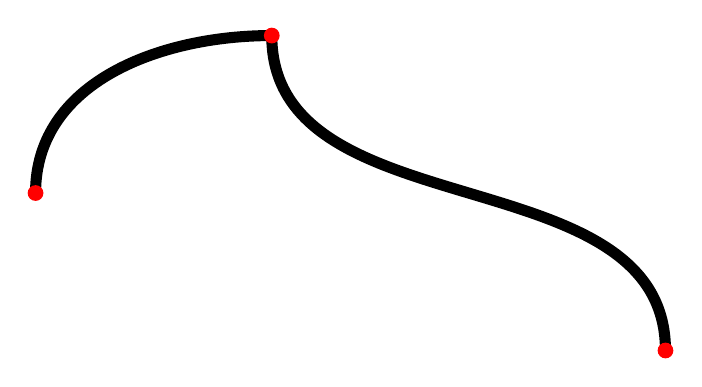
\begin{tikzpicture}
		\draw[line width=4pt] (0,0) to [out=90, in=180] (3,2)to [out=-90, in=90] (8,-2);
		\fill[red] (0,0) circle (.1);
		\fill[red] (3,2) circle (.1);
		\fill[red] (8,-2) circle (.1);
		\end{tikzpicture}
	\end{center}
\end{fragileframe}

%---------------------------------------------------------------------------------------------------------------------------------------- 
\usetikzlibrary{arrows,chains,matrix,positioning,scopes}
\begin{fragileframe}{Flêches et patterns}	
	\begin{center}
		\begin{adjustbox}{max width=\textwidth}
			\begin{tabular}{cl}
				\tikz{\draw[->]              (0,0) -- (2,0);} & \verb+\draw[->]              (0,0) -- (2,0);+ \\
				\tikz{\draw[dotted, >->>]    (0,0) -- (2,0);} & \verb+\draw[dotted, >->>]    (0,0) -- (2,0);+ \\
				\tikz{\draw[|<->|]           (0,0) -- (2,0);} & \verb+\draw[|<->|]           (0,0) -- (2,0);+ \\
				\tikz{\draw[dashed, o-)]     (0,0) -- (2,0);} & \verb+\draw[dashed, o-)]     (0,0) -- (2,0);+ \\
				\tikz{\draw[loosely dashed]  (0,0) -- (2,0);} & \verb+\draw[loosely dashed]  (0,0) -- (2,0);+ \\
				\tikz{\draw[densely dotted]  (0,0) -- (2,0);} & \verb+\draw[densely dotted]  (0,0) -- (2,0);+ \\
				\tikz{\draw[->] (0,0) .. controls (.5,-.5) .. (2, 0);} & \verb+\draw[->] (0,0) .. controls (.5,-.5) .. (2, 0);+ \\
			\end{tabular}
		\end{adjustbox}
	\end{center}
\end{fragileframe}

%---------------------------------------------------------------------------------------------------------------------------------------- 

\begin{fragileframe}{\texttt{clip} et \texttt{scope}}
	
	\begin{itemize}
		\item Après une commande \verb+\clip+,tous les dessins sont aussi "clippés", seulement les parties à l'intérieur de la région coupée sont déssinées.
		\item L'utilisation de l'environnement \texttt{scope} permet de restreindre la portée de ce type de commande :
	\end{itemize}
	
\begin{minipage}[c]{0.45\textwidth}
	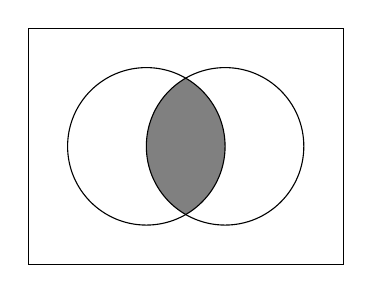
\begin{tikzpicture}
	\draw (-2, 1.5) rectangle (2, -1.5);
	\begin{scope}
	\clip (-0.5, 0) circle (1);
	\clip ( 0.5, 0) circle (1);
	\fill[color=gray] (-2,1.5)rectangle (2,-1.5);
	\end{scope}
	\draw (-0.5, 0) circle (1);
	\draw ( 0.5, 0) circle (1);
	\end{tikzpicture}
\end{minipage}
\begin{minipage}{0.53\textwidth}
\scriptsize
\begin{Verbatim}
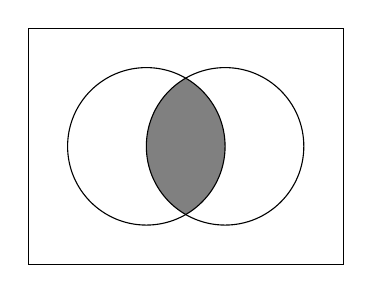
\begin{tikzpicture}
  \draw (-2, 1.5) rectangle (2, -1.5);
  \begin{scope}
    \clip (-0.5, 0) circle (1);
    \clip ( 0.5, 0) circle (1);
    \fill[color=gray] (-2,1.5)rectangle (2,-1.5);
  \end{scope}
  \draw (-0.5, 0) circle (1);
  \draw ( 0.5, 0) circle (1);
\end{tikzpicture}
\end{Verbatim}
\end{minipage}

\end{fragileframe}

%---------------------------------------------------------------------------------------------------------------------------------------- 

\begin{fragileframe}{Nodes}
	
	\begin{itemize}
		\item Les noeuds sont ajoutés après qu'un \texttt{path} soit dessiné:
\begin{minipage}{0.2\textwidth}
\begin{tikzpicture}
\path[draw] (0, 0) node {A} -- (1,0) -- (1,1) node {B};
\end{tikzpicture}
\end{minipage}
\begin{minipage}{0.66\textwidth}
\scriptsize \verb+\path[draw] (0, 0) node {A} -- (1,0) -- (1,1) node {B};+
\end{minipage}		
		
		
		\item Les noeuds peuvent être nommés pour référence future. Ils ont également beaucoup d'options :\\
\begin{minipage}{0.2\textwidth}
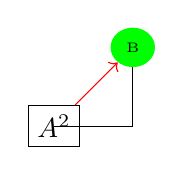
\begin{tikzpicture}
\path[draw] (0, 0) node[draw] (nodeA)  {$A^2$} -- (1,0)-- (1,1) node[ellipse,fill=green](nodeB) {\tiny B};
\draw[red,->] (nodeA) -- (nodeB);
\end{tikzpicture}
\end{minipage}
\begin{minipage}{0.66\textwidth}
\scriptsize
\begin{Verbatim}
\path[draw] (0, 0) node[draw] (nodeA)  {$A^2$} 
	-- (1,0)-- (1,1) node[ellipse,fill=green]
	(nodeB) {\tiny B};
\draw[red,->] (nodeA) -- (nodeB);
\end{Verbatim}
\end{minipage}

		\item Il est souvent préférable de définir d'abord les noeuds nommés, puis de les connecter ultérieurement, car les chemins sont tronqués autour des noeuds:
		\scriptsize\verb+\node[Options] (node name) at (x,y) {TeX content of node}+
	\end{itemize}
\end{fragileframe}

%---------------------------------------------------------------------------------------------------------------------------------------- 

\begin{fragileframe}{}
	
	\begin{minipage}[c]{0.2\textwidth}
		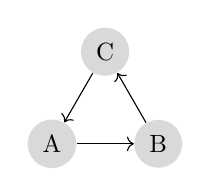
\begin{tikzpicture}[scale=.9, transform shape]
			\tikzstyle{every node} = [circle, fill=gray!30]
			\node (a) at (0, 0) {A};
			\node (b) at +(0: 1.5) {B};
			\node (c) at +(60: 1.5) {C};
			\foreach \from/\to in {a/b, b/c, c/a}
				\draw [->] (\from) -- (\to);
		\end{tikzpicture}
	\end{minipage}
	\begin{minipage}{0.76\textwidth}
		\scriptsize
		\begin{Verbatim}
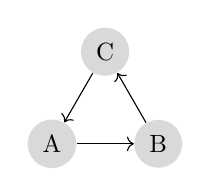
\begin{tikzpicture}[scale=.9, transform shape]
  \tikzstyle{every node} = [circle, fill=gray!30]
  \node (a) at (0, 0) {A};
  \node (b) at +(0: 1.5) {B};
  \node (c) at +(60: 1.5) {C};
  \foreach \from/\to in {a/b, b/c, c/a}
    \draw [->] (\from) -- (\to);
\end{tikzpicture}
		\end{Verbatim}
	\end{minipage}
\vfill

	Note: \texttt{scale} et les autres transformations ne s'appliquent généralement pas sur les noeuds. Si vous souhaitez le faire, il faut ajouter l'option \texttt{transform shape}.
\end{fragileframe}

%---------------------------------------------------------------------------------------------------------------------------------------- 

\begin{fragileframe}{}
	
	\begin{itemize}
		\item Les noeuds sur un \texttt{path} peuvent être optionnellement placés : 
		\begin{minipage}{0.3\textwidth}
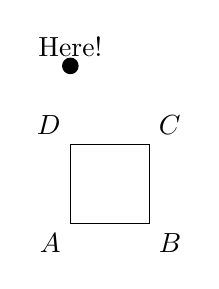
\begin{tikzpicture}
\fill (0,2) circle (3pt) node[above] {Here!};
\draw (0,0) node[below left] {$A$} 
	--(1,0) node[below right] {$B$} 
	--(1,1) node[above right] {$C$} 
	--(0,1) node[above left]  {$D$} 
	-- cycle;
\end{tikzpicture}
		\end{minipage}
		\begin{minipage}{0.56\textwidth}
			\scriptsize 
\begin{Verbatim}
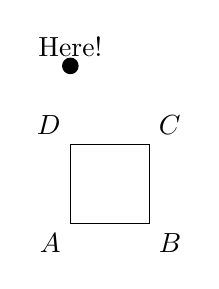
\begin{tikzpicture}
  \fill (0,2) circle (3pt) node[above] {Here!};
  \draw (0,0) node[below left] {$A$} 
    --(1,0) node[below right] {$B$} 
    --(1,1) node[above right] {$C$} 
    --(0,1) node[above left]  {$D$} 
    -- cycle;
\end{tikzpicture}
\end{Verbatim}
		\end{minipage}		
		
		
		\item Les noeuds sur un chemin peuvent aussi êtrê placé par la position proportionnelle au chemin parcouru (\texttt{pos=0} est le début et \texttt{pos=1} est la fin)\\
		\begin{minipage}{0.4\textwidth}
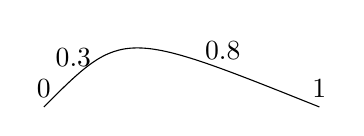
\begin{tikzpicture}
\draw (0,0) .. controls (1,1) .. (3.5, 0)
	node[pos=0,above] {0}
	node[pos=.3, left] {0.3}
	node[pos=0.8,above]{0.8}
	node[pos=1,above]{1};
\end{tikzpicture}
		\end{minipage}
		\begin{minipage}{0.46\textwidth}
			\scriptsize
			\begin{Verbatim}
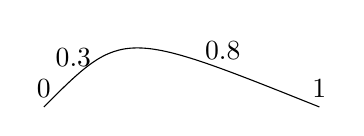
\begin{tikzpicture}
\draw (0,0) .. controls (1,1) .. (3.5, 0)
  node[pos=0,above] {0}
  node[pos=.3, left] {0.3}
  node[pos=0.8,above]{0.8}
  node[pos=1,above]{1};
\end{tikzpicture}
			\end{Verbatim}
		\end{minipage}
	\end{itemize}
\end{fragileframe}

%---------------------------------------------------------------------------------------------------------------------------------------- 

\begin{fragileframe}{D'autres exemples}
	
		\begin{minipage}{0.2\textwidth}
			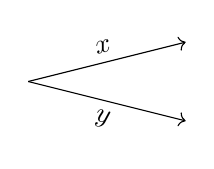
\begin{tikzpicture}
			\draw[->] (0,0) -- (2,0.5) node[pos=.5,sloped,above] {$x$};
			\draw[->] (0,0) -- (2,-.5) node[pos=.5,sloped,below] {$y$};
			\end{tikzpicture}
		\end{minipage}
		\begin{minipage}{0.76\textwidth}
			\scriptsize 
\begin{Verbatim}
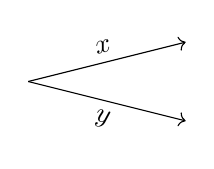
\begin{tikzpicture}
  \draw[->] (0,0) -- (2,0.5) node[pos=.5,sloped,above] {$x$};
  \draw[->] (0,0) -- (2,-.5) node[pos=.5,sloped,below] {$y$};
\end{tikzpicture}
\end{Verbatim}
		\end{minipage}		

		\begin{minipage}{0.2\textwidth}
			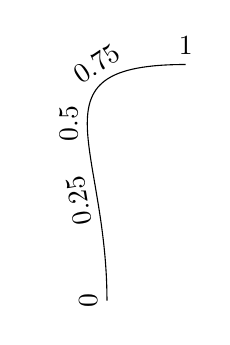
\begin{tikzpicture}
			\tikzstyle{every node} = [sloped,above, allow upside down]
			\draw (0,0).. controls +(up:2cm) and +(left:2cm) ..(1,3)
			\foreach \p in {0,0.25,...,1} {node[pos=\p]{\p}};
			\end{tikzpicture}
		\end{minipage}
		\begin{minipage}{0.46\textwidth}
			\scriptsize
\begin{Verbatim}
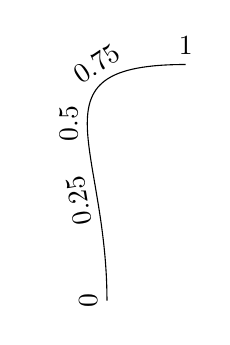
\begin{tikzpicture}
  \tikzstyle{every node} = [sloped,above, allow upside down]
  \draw (0,0).. controls +(up:2cm) and +(left:2cm) ..(1,3)
  \foreach \p in {0,0.25,...,1} {node[pos=\p]{\p}};
\end{tikzpicture}
\end{Verbatim}
		\end{minipage}

\end{fragileframe}

%---------------------------------------------------------------------------------------------------------------------------------------- 

\begin{fragileframe}{}
	
	Des calculs simples sont aussi possibles : 
	
	\vfill
	\begin{minipage}{0.3\textwidth}
		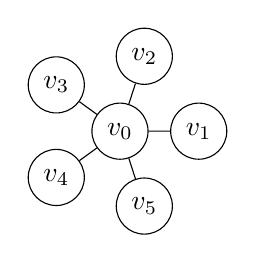
\begin{tikzpicture}
			\tikzstyle{every node}=[draw,shape=circle];
			\node (v0) at (0:0) {$v_0$};
			\node (v1) at (   0:1) {$v_1$};
			\node (v2) at (  72:1) {$v_2$};
			\node (v3) at (2*72:1) {$v_3$};
			\node (v4) at (3*72:1) {$v_4$};
			\node (v5) at (4*72:1) {$v_5$};
			\draw (v0) -- (v1)(v0) -- (v2)(v0) -- (v3)(v0) -- (v4)(v0) -- (v5);
		\end{tikzpicture}
	\end{minipage}
	\begin{minipage}{0.66\textwidth}
		\scriptsize 
		\begin{Verbatim}
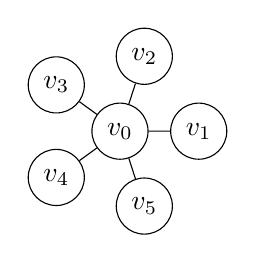
\begin{tikzpicture}
  \tikzstyle{every node}=[draw,shape=circle];
  \node (v0) at (0:0) {$v_0$};
  \node (v1) at (   0:1) {$v_1$};
  \node (v2) at (  72:1) {$v_2$};
  \node (v3) at (2*72:1) {$v_3$};
  \node (v4) at (3*72:1) {$v_4$};
  \node (v5) at (4*72:1) {$v_5$};
  \draw (v0) -- (v1)
  	(v0) -- (v2)
  	(v0) -- (v3)
  	(v0) -- (v4)
  	(v0) -- (v5);
\end{tikzpicture}
		\end{Verbatim}
	\end{minipage}		
	
\end{fragileframe}

%---------------------------------------------------------------------------------------------------------------------------------------- 

\usetikzlibrary{calc,through}
\begin{fragileframe}{}

\begin{center}
	\begin{tikzpicture}[scale=1.2]
\coordinate [label=left:$A$] (A) at (0,0);
\coordinate [label=right:$B$] (B) at (1.25,0.25);
\draw (A) -- (B);
\node (D) [draw,circle through=(B),label=left:$D$] at (A) {};
\node (E) [draw,circle through=(A),label=right:$E$] at (B) {};
\coordinate[label=above:$C$] (C) at (intersection 2 of D and E);
\draw [red] (A) -- (C);\draw [red] (B) -- (C);
\end{tikzpicture}
\end{center}

		\scriptsize 
		\begin{Verbatim}
\usetikzlibrary{calc,through}

\begin{tikzpicture}[scale=1.2]
	\coordinate [label=left:$A$] (A) at (0,0);
	\coordinate [label=right:$B$] (B) at (1.25,0.25);
	\draw (A) -- (B);
	\node (D) [draw,circle through=(B),label=left:$D$] at (A) {};
	\node (E) [draw,circle through=(A),label=right:$E$] at (B) {};
	\coordinate[label=above:$C$] (C) at (intersection 2 of D and E);
	\draw [red] (A) -- (C);\draw [red] (B) -- (C);
\end{tikzpicture}
		\end{Verbatim}
	
\end{fragileframe}

%---------------------------------------------------------------------------------------------------------------------------------------- 

\begin{fragileframe}{Boucles \texttt{foreach}}

\begin{center}
	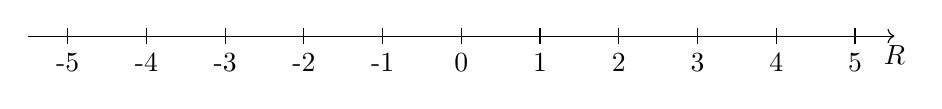
\begin{tikzpicture}
	\draw[->] (-5.5,0) -- (5.5,0) node [below] {$\mathbb{R}$}; 
	\foreach \x in {-5,...,5} 
		\draw (\x, 0.1) -- (\x, -0.1) node [below] {\x};
	\end{tikzpicture}
	
	\scriptsize 
\begin{Verbatim}
\draw[->] (-5.5,0) -- (5.5,0) node [below] {$\mathbb{R}$}; 
\foreach \x in {-5,...,5} 
  \draw (\x, 0.1) -- (\x, -0.1) node [below] {\x};
\end{Verbatim}
\end{center}


	
\begin{center}
	\begin{tikzpicture}
	\foreach \x in {1,2,...,10} 
		\shade[ball color=ulred!\x 0!ulgold] (\x,0) circle (3mm);
	\end{tikzpicture}
	
	\scriptsize 
\begin{Verbatim}
\foreach \x in {1,3,...,10} 
  \shade[ball color=ulred!\x 0!ulgold] (\x,0) circle (3mm);
\end{Verbatim}
\end{center}

\begin{center}
	\begin{tikzpicture}
	\foreach \x in {9,...,1} 
		\draw[fill=ulblue!\x0] (-0.1*\x - 1, -0.1*\x ) 
			rectangle (0.1*\x + 1, 0.1*\x );
	\end{tikzpicture}
	
	\scriptsize 
\begin{Verbatim}
\foreach \x in {9,...,1} 
  \draw[fill=ulblue!\x0] (-0.1*\x - 1, -0.1*\x ) 
    rectangle (0.1*\x + 1, 0.1*\x );
\end{Verbatim}
\end{center}

\end{fragileframe}

%---------------------------------------------------------------------------------------------------------------------------------------- 

% For every picture that defines or uses external nodes, you'll have to
% apply the 'remember picture' style. To avoid some typing, we'll apply
% the style to all pictures.
\tikzstyle{every picture}+=[remember picture]

\begin{fragileframe}{Réferences et \texttt{overlay}}
	\begin{itemize}
		\item Ajouter \verb|\tikzstyle{every picture}+=[remember picture]| dans le préambule
		\item Ajouter l'option \texttt{overlay} à tous les \tikz[baseline,inner sep=0]{\node[anchor=base] (n1) {\texttt{paths}};} qui utilisent des noeuds référencés dans d'autres images TikZ
		\item Il faudra peut-être recompiler deux fois (selon l'IDE)
		\item le mot "\tikz[baseline,inner sep=0]{\node[anchor=base] (n2) {\texttt{paths}};}" ci-dessus est en fait un noeud :  \\
		\scriptsize
			\begin{Verbatim}
... à tous les \tikz{[baseline,inner sep=0] 
\node[anchor=base] (n1) {paths};} qui utilisent ...
\end{Verbatim}
		\normalsize
		\item Et enfin nous dessinons la flêche : \verb+\tikz[overlay]{\draw[thick,ulred,->] (n2) -- (n1);}+ 
		\scriptsize\tikz[overlay]{\draw[thick,ulred,->] (n2) -- (n1);}
	\end{itemize}
	
\end{fragileframe}


%---------------------------------------------------------------------------------------------------------------------------------------- 

\begin{frame}[fragile]{Intégration a Beamer}

\[
y = \tikz[baseline]{\node[fill=ulblue!50,anchor=base] (t1){$a$};} 
	x +\tikz[baseline]{\node[fill=ulred!50,anchor=base ] (t2){$b$};}
\] 

\begin{itemize}
	\item[]<2-> \tikz{\node [fill=ulblue!50,draw,circle] (n1) {};} slope
	\item[]<3-> \tikz{\node [fill=ulred!50,draw,circle] (n2) {};} y-intercept
\end{itemize} 

\begin{tikzpicture}[overlay]
	\path<4->[ulblue!50,->] (n1.north) edge [out= 60, in= 135] (t1.north west);
	\path<5>[ulred!50,->] (n2.south) edge [out=-70, in=-110] (t2.south);
\end{tikzpicture} 

\scriptsize 
\begin{Verbatim} 
\[
 y = \tikz[baseline]{\node[fill=blue!50,anchor=base] (t1){$a$};} 
   x +\tikz[baseline]{\node[fill=red!50,anchor=base ] (t2){$b$};}
\] 
\begin{itemize} 
  \item[]<2-> \tikz\node [fill=blue!50,draw,circle] (n1) {}; slope
  \item[]<3-> \tikz\node [fill=red!50,draw,circle] (n2) {}; y-intercept
\end{itemize} 
\begin{tikzpicture}[overlay]
  \path<4->[blue,->] (n1.north) edge [out= 60, in= 135] (t1.north west);
  \path<5>[red,->] (n2.south) edge [out=-70, in=-110] (t2.south)
\end{tikzpicture} 
\end{Verbatim} 
	
\end{frame}

%---------------------------------------------------------------------------------------------------------------------------------------- 

\tikzset{
	treenode/.style = {shape=rectangle, rounded corners,
		draw, align=center,
		top color=white, bottom color=ulblue!20},
	root/.style     = {treenode, font=\Large, bottom color=red!30},
	env/.style      = {treenode, font=\ttfamily\normalsize},
	dummy/.style    = {circle,draw}
}
\usetikzlibrary{mindmap,trees,shapes,decorations}
\begin{frame}[fragile]{Quelques librairies utiles de TikZ}
Shapes : 

\begin{center}
	\begin{adjustbox}{max height=.8\textheight}
		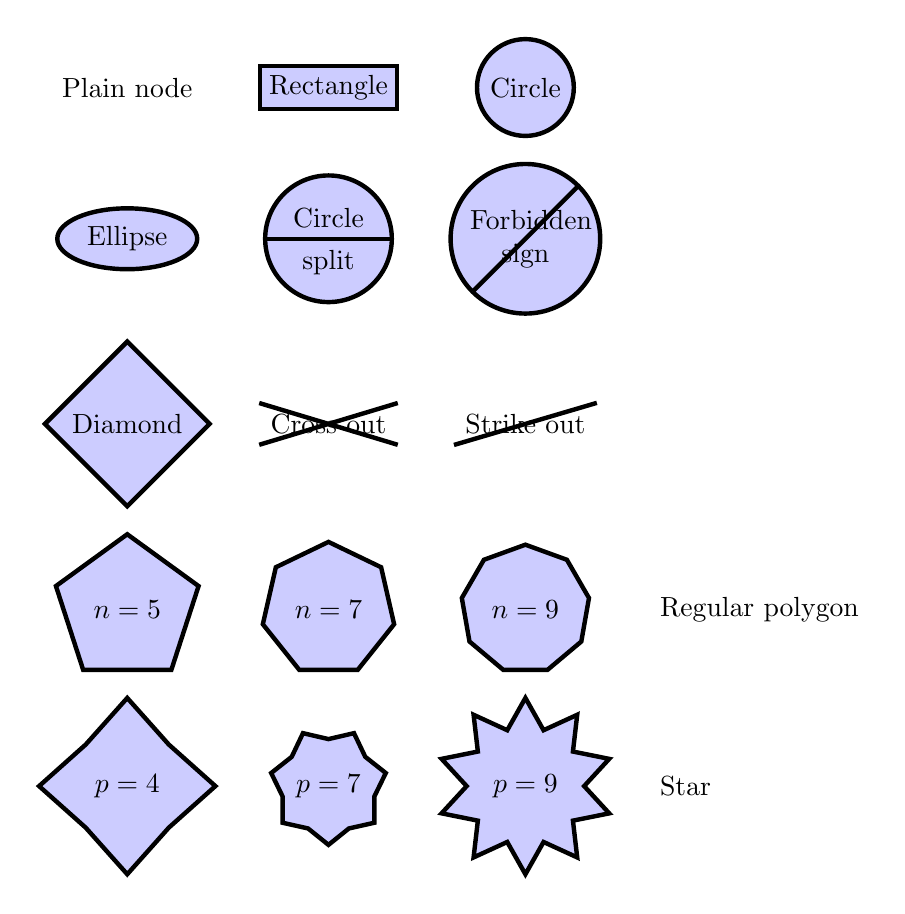
\begin{tikzpicture}[scale=2]
		\tikzstyle{ann}=[draw=none,fill=none,right]
		\matrix[nodes={draw, ultra thick, fill=blue!20},row sep=0.3cm,column sep=0.5cm] 
		{
			\node[draw=none,fill=none] {Plain node}; & \node[rectangle] {Rectangle}; & \node[circle] {Circle};\\
			\node[ellipse] {Ellipse};& \node[circle split] {Circle \nodepart{lower} split};& \node[forbidden sign,text width=4em, text centered]{Forbidden sign};\\
			\node[diamond] {Diamond};& \node[cross out] {Cross out};& \node[strike out] {Strike out};\\
			\node[regular polygon,regular polygon sides=5] {$n=5$};& \node[regular polygon,regular polygon sides=7] {$n=7$};& \node[regular polygon,regular polygon sides=9] {$n=9$};& \node[ann]{Regular polygon};\\
			\node[star,star points=4] {$p=4$};& \node[star,star points=7,star point ratio=0.8] {$p=7$};& \node[star,star points=10] {$p=9$};& \node[ann]{Star};\\
		};
		\end{tikzpicture}
	\end{adjustbox}
\end{center}				
\end{frame}
%---------------------------------------------------------------------------------------------------------------------------------------- 
\begin{frame}{Quelques librairies utiles de TikZ}
		Trees :
		
	\begin{adjustbox}{max width=\textwidth}
		\begin{tikzpicture}
		[
		grow                    = right,
		sibling distance        = 6em,
		level distance          = 10em,
		edge from parent/.style = {draw, -latex},
		every node/.style       = {font=\footnotesize},
		sloped
		]
		\node [root] {Formula}
		child { node [env] {equation}
			edge from parent node [below] {single-line?} }
		child { node [dummy] {}
			child { node [dummy] {}
				child { node [env] {align\\flalign}
					edge from parent node [below] {at relation sign?} }
				child { node [env] {alignat}
					edge from parent node [above] {at several}
					node [below] {places?} }
				child { node [env] {gather}
					edge from parent node [above] {centered?} }
				edge from parent node [below] {aligned?} }
			child { node [env] {multline}
				edge from parent node [above, align=center]
				{first left,\\centered,}
				node [below] {last right}}
			edge from parent node [above] {multi-line?} };
		\end{tikzpicture}
	\end{adjustbox}
		
\end{frame}
%---------------------------------------------------------------------------------------------------------------------------------------- 
\begin{frame}{Quelques librairies utiles de TikZ}
		MindMaps : 
		
\begin{center}
		\begin{adjustbox}{max height=.8\textheight}
		\begin{tikzpicture}
		\path[mindmap,concept color=black,text=white]
		node[concept] {Computer Science}
		[clockwise from=0]
		child[concept color=green!50!black] {
			node[concept] {practical}
			[clockwise from=90]
			child { node[concept] {algorithms} }
			child { node[concept] {data structures} }
			child { node[concept] {pro\-gramming languages} }
			child { node[concept] {software engineer\-ing} }
		}  
		child[concept color=blue] {
			node[concept] {applied}
			[clockwise from=-30]
			child { node[concept] {databases} }
			child { node[concept] {WWW} }
		}
		child[concept color=red] { node[concept] {technical} }
		child[concept color=orange] { node[concept] {theoretical} };
		\end{tikzpicture}
	\end{adjustbox}
\end{center}	
	
\end{frame}

%---------------------------------------------------------------------------------------------------------------------------------------- 
\begin{frame}{Quelques librairies utiles de TikZ}
	
Automatas, calendar, decorations, matrix, shadows, functions and data plots, ... google \texttt{usetikzlibrary}

\begin{center}
	\begin{tikzpicture}
		\draw[thick] (0,0) circle (1);
		\draw[thick] plot [smooth,tension=1.5] coordinates{(-0.3,-0.5) (0,-0.7) (0.3,-0.5)};
		\draw [thick, fill=black] (0,-0.2) circle (0.1);
		\node[circle,minimum width=0.1, inner color=ulred] at (-0.6,-0.2) {};
		\node[circle,minimum width=0.1, inner color=ulred] at (0.6,-0.2) {};
		\draw [rotate=90, fill=black] (0.3,0.3) ellipse (0.2 and 0.1);
		\draw [rotate=90, fill=black] (0.3,-0.3) ellipse (0.2 and 0.1);
	\end{tikzpicture}
\end{center}

\end{frame}


%---------------------------------------------------------------------------------------------------------------------------------------- 
% Define a the counter cnt. Used to identify files generated for use
% with Gnuplot.
\newcounter{cnt}
\setcounter{cnt}{0}

\newcommand{\distpic}[3]{
    % First draw the upper distribution.
    % Shade the critical region:
    \fill[red!30] (0.658,0)  -- plot[id=f3,domain=0.658:3,samples=50]
        function {exp(-x*x*0.5/0.16)} -- (3,0) -- cycle;

    % Draw the normal distribution curve
    \draw[blue!50!black,smooth,thick] plot[id=f1,domain=-2:3,samples=50]
    function {exp(-x*x*0.5/0.16)};
    % Draw the x-axis
    \draw[->,black] (-2.2,0) -- (3.2,0);
    % Put some ticks and tick labels in:
    \foreach \x in {-2,-1,0,1,2,3}
    \draw (\x,0) -- (\x,-0.1) node[below] {$\x$};
    % Put in a label for the critical region boundary:
    \draw[red!50!black,thick] (0.658,0) node[below,yshift=-0.5cm] {0.658}
    -- (0.658,0.85);

    % Put in labels for accepting or rejecting the null hypothesis with
    % the corresponding regions:
    \draw[red!50!black,thick,->] (0.688,0.7) -- (1.3,0.7)
        node[anchor=south] {Reject  $H_0$};
    \draw[red!50!black,thick,->] (0.628,0.7) -- (-1,0.7)
        node[anchor=south]{\parbox{1.5cm}{\raggedright Fail to reject $H_0$}};

    % Add a label to the upper picture, when the null is true
    \draw (-3,1) node[above,draw,fill=green!30] {$H_0$ is true:};

    % Label the critical region with an alpha level:
    \draw[<-,thick] (0.75,0.05) -- (1.6,0.2) node[right,yshift=0.3cm]
    {\begin{tabular}{l} $\alpha=0.05$ \\ (Type I error rate) \end{tabular}};


    % Add a label showing the effect size between the two plots:
    \draw[very thin] (0,-1) -- (0,-0.5);
    \draw[<->,thick] (0,-1) node[left] {Effect size:  #1} -- (#1,-1);
    \draw[thick] (0,-.9) -- (0,-1.1);

    \draw[very thin] (#1,-1) -- (#1,-1.7);
    \draw[thick] (#1,-.9) -- (#1,-1.1);

    % Now draw the lower distribution showing the effect size:
    \begin{scope}[yshift=-3cm]
    % Shade the "reject H0" region red
    \fill[red!30] (0.658,0)  -- plot[id=f3\thecnt,domain=0.658:3,samples=50]
        function {exp(-(x-#1)*(x-#1)*0.5/0.16)} --
        (3,0) -- cycle;
        % Shade the "accept H0" region blue
    \fill[blue!30] (-2,0) -- plot[id=f4\thecnt,domain=-2:0.658,samples=50]
        function {exp(-(x-#1)*(x-#1)*0.5/0.16)} --
        (0.658,0) -- cycle;

        % Draw the shifted normal distribution:
    \draw[blue!50!black,smooth,thick] plot[id=f1\thecnt,domain=-2:3,samples=50]
            function {exp(-(x-#1)*(x-#1)*0.5/0.16)};

        % Draw the x-axis and put in some ticks and tick labels
    \draw[->,black] (-2.2,0) -- (3.2,0);
    \foreach \x in {-2,-1,0,1,2,3}
            \draw (\x,0) -- (\x,-0.1) node[below] {$\x$};

        % Draw and label the critical region boundary
    \draw[red!50!black,very thick] (0.658,0) node[below,yshift=-0.5cm] {0.658}
        -- (0.658,1.0);
    \draw[red!50!black,very thick,->] (0.688,0.7) -- (2.7,0.7)
        node[anchor=south west] {Reject  $H_0$};
    \draw[red!50!black,very thick,->] (0.628,0.7) -- (-0.5,0.7)
        node[anchor=south]{\parbox{1.5cm}{\raggedright Fail to reject $H_0$}};

    % Add a label to the lower picture, when the alternative hypothesis is true:
    \draw (-3,1) node[above,draw,fill=green!30] {$H_a$ is true:};

        % Add labels showing the statistical power and the Type II error rate:
    \draw[<-,thick] (1.5,0.1) -- (3,0.2) node[anchor=south west]
        {Power = \large #2};
    \draw[<-,thick] (0.4,0.1) -- (-1,0.2) node[left,yshift=0.3cm]
        {\begin{tabular}{l}
        $\beta$ = {\large #3} \\ (Type II error rate) \end{tabular}};
    \end{scope}
}
\begin{frame}{Animations en TikZ}
Puissance statistique dans les tests d'hypothèses:

\begin{animateinline}[autoplay,loop,begin={\begin{tikzpicture}[scale=1.3]},end={\stepcounter{cnt}\end{tikzpicture}}]{3}
	\distpic{0.5}{.346}{.654}\newframe
	\distpic{0.7}{.542}{.458}\newframe
	\distpic{0.9}{.727}{.273}\newframe
	\distpic{1.1}{.865}{.135}\newframe
	\distpic{1.3}{.946}{.054}\newframe
	\distpic{1.5}{.982}{.018}\newframe
	\distpic{1.7}{.995}{.005}\newframe
	\distpic{1.9}{.999}{.001}
\end{animateinline}
\end{frame}


%---------------------------------------------------------------------------------------------------------------------------------------- 
\begin{frame}{Liens utiles \LaTeX / \texttt{tikz}}

\begin{itemize}
	\item Ressources web : 
	\begin{itemize}
	\item \url{http://www.texample.net/tikz/resources/}
	\item \url{http://www.texample.net/tikz/examples/}
	\end{itemize}
	\item Editeurs \texttt{tikz} graphiques (pour un début)
	\begin{itemize}
	\item \url{http://www.tikzedt.org/}
	\item \url{https://tikzit.github.io}/
	\end{itemize}
	\item Réseaux de neurones \texttt{tikz}
	\begin{itemize}
	\item \url{https://github.com/HarisIqbal88/PlotNeuralNet}
	\item \url{https://github.com/PetarV-/TikZ}
	\end{itemize}
\end{itemize}

\end{frame}

%---------------------------------------------------------------------------------------------------------------------------------------- 
\usetikzlibrary{arrows,decorations.pathmorphing,backgrounds,positioning,fit,petri, decorations.pathreplacing,shadows,calc}

\definecolor{echoreg}{HTML}{2cb1e1}
\definecolor{mymauve}{rgb}{0.58,0,0.82}

\newtoggle{redraw}
\newtoggle{redraw2}

\tikzset{%
	pics/cube/.style args={#1/#2/#3/#4}{code={%
			\begin{scope}[line width=#4mm]
				\begin{scope}
					\clip (-#1,-#2,0) -- (#1,-#2,0) -- (#1,#2,0) -- (-#1,#2,0) -- cycle;
					\filldraw (-#1,-#2,0) -- (#1,-#2,0) -- (#1,#2,0) -- (-#1,#2,0) -- cycle;
				\end{scope}
				\iftoggle{redraw}{%
				}{%
					\begin{scope}
						\clip (-#1,-#2,0) -- (-#1-#3,-#2,-#3) -- (-#1-#3,#2,-#3) -- (-#1,#2,0) -- cycle;
						\filldraw (-#1,-#2,0) -- (-#1-#3,-#2,-#3) -- (-#1-#3,#2,-#3) -- (-#1,#2,0) -- cycle;
					\end{scope}
				}
				\iftoggle{redraw2}{%
				}{
					\begin{scope}
						\clip (-#1,#2,0) -- (-#1-#3,#2,-#3) -- (#1-#3,#2,-#3) -- (#1,#2,0) -- cycle;
						\filldraw (-#1,#2,0) -- (-#1-#3,#2,-#3) -- (#1-#3,#2,-#3) -- (#1,#2,0) -- cycle;
					\end{scope}
				}
				\node[inner sep=0] (-A) at (-#1-#3*0.5, 0, -#3*0.5) {};
				\node[inner sep=0] (-B) at (#1-#3*0.5, 0, -#3*0.5) {};
				
				\coordinate (-V) at (#1, #2);
				\coordinate (-W) at (#1, -#2);
			\end{scope}
}}}

\begin{frame}{Un CNN ?}

\begin{adjustbox}{max width=\textwidth}
\begin{tikzpicture}
\input{xcnn.tikz}
\end{tikzpicture}
\end{adjustbox}

\tiny
Source : \url{https://github.com/PetarV-/TikZ}
\end{frame}


%---------------------------------------------------------------------------------------------------------------------------------------- 
\newcommand{\empt}[2]{$#1^{\langle #2 \rangle}$}
\begin{frame}[label=conclu]{Conclusion}
\begin{center}
	\Huge{That's all folks !}

\resizebox{!}{.5\textheight}{
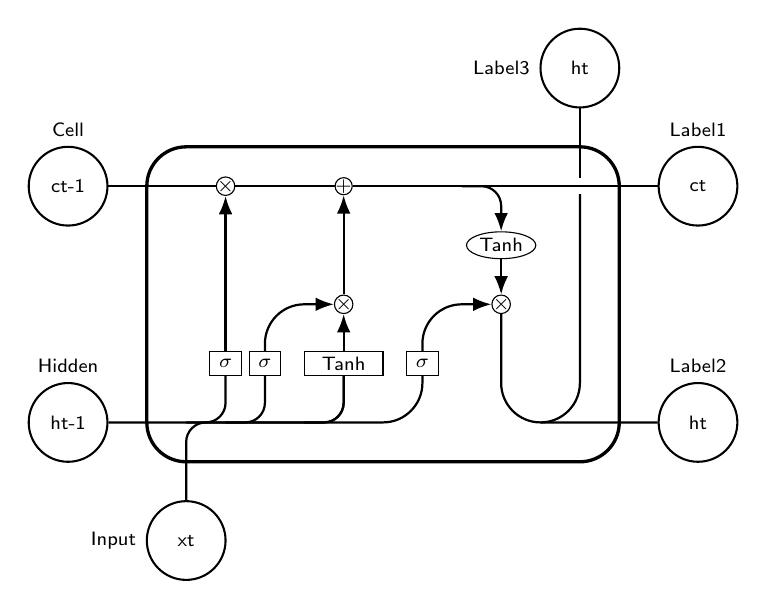
\begin{tikzpicture}[
% GLOBAL CFG
font=\sf \scriptsize,
>=LaTeX,
% Styles
cell/.style={% For the main box
	rectangle, 
	rounded corners=5mm, 
	draw,
	very thick,
},
operator/.style={%For operators like +  and  x
	circle,
	draw,
	inner sep=-0.5pt,
	minimum height =.2cm,
},
function/.style={%For functions
	ellipse,
	draw,
	inner sep=1pt
},
ct/.style={% For external inputs and outputs
	circle,
	draw,
	line width = .75pt,
	minimum width=1cm,
	inner sep=1pt,
},
gt/.style={% For internal inputs
	rectangle,
	draw,
	minimum width=4mm,
	minimum height=3mm,
	inner sep=1pt
},
mylabel/.style={% something new that I have learned
	font=\scriptsize\sffamily
},
ArrowC1/.style={% Arrows with rounded corners
	rounded corners=.25cm,
	thick,
},
ArrowC2/.style={% Arrows with big rounded corners
	rounded corners=.5cm,
	thick,
},
]

%Start drawing the thing...    
% Draw the cell: 
\node [cell, minimum height =4cm, minimum width=6cm] at (0,0){} ;

% Draw inputs named ibox#
\node [gt] (ibox1) at (-2,-0.75) {$\sigma$};
\node [gt] (ibox2) at (-1.5,-0.75) {$\sigma$};
\node [gt, minimum width=1cm] (ibox3) at (-0.5,-0.75) {Tanh};
\node [gt] (ibox4) at (0.5,-0.75) {$\sigma$};

% Draw opérators   named mux# , add# and func#
\node [operator] (mux1) at (-2,1.5) {$\times$};
\node [operator] (add1) at (-0.5,1.5) {+};
\node [operator] (mux2) at (-0.5,0) {$\times$};
\node [operator] (mux3) at (1.5,0) {$\times$};
\node [function] (func1) at (1.5,0.75) {Tanh};

% Draw External inputs? named as basis c,h,x
\node[ct, label={[mylabel]Cell}] (c) at (-4,1.5) {\empt{c}{t-1}};
\node[ct, label={[mylabel]Hidden}] (h) at (-4,-1.5) {\empt{h}{t-1}};
\node[ct, label={[mylabel]left:Input}] (x) at (-2.5,-3) {\empt{x}{t}};

% Draw External outputs? named as basis c2,h2,x2
\node[ct, label={[mylabel]Label1}] (c2) at (4,1.5) {\empt{c}{t}};
\node[ct, label={[mylabel]Label2}] (h2) at (4,-1.5) {\empt{h}{t}};
\node[ct, label={[mylabel]left:Label3}] (x2) at (2.5,3) {\empt{h}{t}};

% Start connecting all.
%Intersections and displacements are used. 
% Drawing arrows    
\draw [ArrowC1] (c) -- (mux1) -- (add1) -- (c2);

% Inputs
\draw [ArrowC2] (h) -| (ibox4);
\draw [ArrowC1] (h -| ibox1)++(-0.5,0) -| (ibox1); 
\draw [ArrowC1] (h -| ibox2)++(-0.5,0) -| (ibox2);
\draw [ArrowC1] (h -| ibox3)++(-0.5,0) -| (ibox3);
\draw [ArrowC1] (x) -- (x |- h)-| (ibox3);

% Internal
\draw [->, ArrowC2] (ibox1) -- (mux1);
\draw [->, ArrowC2] (ibox2) |- (mux2);
\draw [->, ArrowC2] (ibox3) -- (mux2);
\draw [->, ArrowC2] (ibox4) |- (mux3);
\draw [->, ArrowC2] (mux2) -- (add1);
\draw [->, ArrowC1] (add1 -| func1)++(-0.5,0) -| (func1);
\draw [->, ArrowC2] (func1) -- (mux3);

%Outputs
\draw [-, ArrowC2] (mux3) |- (h2);
\draw (c2 -| x2) ++(0,-0.1) coordinate (i1);
\draw [-, ArrowC2] (h2 -| x2)++(-0.5,0) -| (i1);
\draw [-, ArrowC2] (i1)++(0,0.2) -- (x2);

\end{tikzpicture}}

	\normalsize Questions ?
\end{center}
\end{frame}



% End of slides
\end{document}